%%%%%%%%%%%%%%%%%%%%%%%%%%%%%%%%%%%%%%%%%%%%%%%%%%%%%%%%%%%%%%%%%%%%%%%%%%%%%%
% This is just an example/guide for you to refer to when submitting
% manuscripts to Frontiers, it is not mandatory to use Frontiers .cls files
% nor frontiers.tex  %
% This will only generate the Manuscript, the final article will be typeset by
% Frontiers after acceptance.
%
% When submitting your files, remember to upload this *tex file, the pdf
% generated with it, the *bib file (if bibliography is not within the *tex)
% and all the figures.
%%%%%%%%%%%%%%%%%%%%%%%%%%%%%%%%%%%%%%%%%%%%%%%%%%%%%%%%%%%%%%%%%%%%%%%%%%%%%%

%%% Version 3.4 Generated 2022/06/14 %%%
%%% You will need to have the following packages installed: datetime,
%%% fmtcount, etoolbox, fcprefix, which are normally inlcuded in WinEdt.
%%% In http://www.ctan.org/ you can find the packages and how to install them,
%%% if necessary.
%%% NB logo1.jpg is required in the path in order to correctly compile front
%%% page header

% for articles in journals using the Harvard Referencing Style (Author-Date),
% for Frontiers Reference Styles by Journal: https://zendesk.frontiersin.org/hc/en-us/articles/360017860337-Frontiers-Reference-Styles-by-Journal
\documentclass[utf8]{FrontiersinHarvard}
% for articles in journals using the Vancouver Reference Style (Numbered), for
% Frontiers Reference Styles by Journal: https://zendesk.frontiersin.org/hc/en-us/articles/360017860337-Frontiers-Reference-Styles-by-Journal
%\documentclass[utf8]{FrontiersinVancouver}
% Vancouver Reference Style (Numbered) for articles in the journals "Frontiers
% in Physics" and "Frontiers in Applied Mathematics and Statistics"
%\documentclass[utf8]{frontiersinFPHY_FAMS}

\usepackage{
    url,
    hyperref,
    lineno,
    microtype,
    subcaption,
    booktabs,
    paralist,
    tablefootnote
}

\usepackage[onehalfspacing]{setspace}

% Hyperref
\hypersetup{
    pdfpagelabels=true,
    plainpages=false,
%    pdfauthor={Author(s)},
    pdftitle={Title},
    pdfsubject={Subject},
    bookmarksnumbered=true,
%    colorlinks,
%    citecolor=black,
%    filecolor=black,
%    linkcolor=black,
%    urlcolor=black,
    pdfstartview=FitH
}

% Bibliography
%\AtEveryBibitem{
%    \clearfield{note}
%    \clearlist{language}
%    \clearfield{isbn}
%%    \clearfield{doi}
%}

%%%%%%%%%%%%%%%%%%%%%%%%%%%%%%%%%%%%%%%%%%%%%%%
% Code listings
%%%%%%%%%%%%%%%%%%%%%%%%%%%%%%%%%%%%%%%%%%%%%%%
\usepackage{inconsolata}

% Code listings with package minted. Requires python
%   pyenv virtualenv 3.x.x myenv
%   pyenv activate myenv
%   pip install pygments
% Then add compilation flag -shell-escape
\usepackage[outputdir=out,newfloat]{minted}
%\usepackage[outputdir=out]{minted}

\usepackage[skins, breakable]{tcolorbox}
\tcbuselibrary{minted}

% Code listing, e.g.
%
%     \begin{codelisting}{
%         \texttt{update} method of the networked audio client implementation,
%         minted style=xcode,
%         minted language=cpp,
%         label=ls:njc-update,
%         float=h!
%     }
%         void NetJUCEClient::update(void) {
%             doAudioOutput();
%
%             handleAudioInput();
%         }
%     \end{codelisting}
\newtcblisting[auto counter]{codelisting}[1]{%
    enhanced,
%    breakable,
%    colback=backcolour,
%    colframe=captioncolor,
    fonttitle=\bfseries\normalsize,
    listing only,
    sharp corners,
    bottomrule=1pt,
    toprule=2pt,
    leftrule=0pt,
    rightrule=0pt,
    title=Listing \thetcbcounter: #1,
    minted style=xcode,
    minted options={
%        fontsize=\footnotesize,
        autogobble
    }
}

% Input code from file, e.g.
%
%       \codeinputlisting[float=h]
%          {text}
%          {listings/udp-packet.txt}
%          {Network capture: ethernet frame containing a UDP packet}
%          {packet-hello-world}
\newtcbinputlisting[use counter from=codelisting]{\codeinputlisting}[5][]{
    minted language=#2,
    listing file={#3},
    title=Listing \thetcbcounter: #4,
    label=listing:#5,
    enhanced,
%    breakable,
%    colback=backcolour,
%    colframe=captioncolor,
    fonttitle=\bfseries\normalsize,
    listing only,
    sharp corners,
    bottomrule=1pt,
    toprule=2pt,
    leftrule=0pt,
    rightrule=0pt,
    minted style=xcode,
    minted options={
%        fontsize=\footnotesize,
        autogobble
    },#1
}

%%%%%%%%%%%%%%%%%%%%%%%%%%%%%%%%%%%%%%%%%%%%%%%%
% SI Units
%%%%%%%%%%%%%%%%%%%%%%%%%%%%%%%%%%%%%%%%%%%%%%%%
%\usepackage[binary-units]{siunitx}
\usepackage{siunitx}
\sisetup{detect-all}

%%%%%%%%%%%%%%%%%%%%%%%%%%%%%%%%%%%%%%%%%%%%%%%%
% TODOS
%%%%%%%%%%%%%%%%%%%%%%%%%%%%%%%%%%%%%%%%%%%%%%%%
\usepackage[
%    disable, %turn off todonotes
    colorinlistoftodos, %enable a coloured square in the list of todos
    textwidth=\marginparwidth, %set the width of the todonotes
    textsize=scriptsize, %size of the text in the todonotes
]{todonotes}

\def\keyFont{\fontsize{8}{11}\helveticabold }

% Internal refs
\newcommand{\figref}[1]{Figure~\ref{#1}}
\newcommand{\figsref}[2]{Figures~\ref{#1} and~\ref{#2}}
\newcommand{\tabref}[1]{Table~\ref{#1}}
\newcommand{\secref}[1]{section~\ref{#1}}
\newcommand{\lstref}[1]{Listing~\ref{#1}}

% Number with base 10 postfix subscript
\newcommand{\numDec}[1]{\num{#1}\textsubscript{10}}

%%%%%%%%%%%%%%%%%%%%%%%%%%%%%%%%%%%%%%%%%%%%%%%%
% Math definitions
%%%%%%%%%%%%%%%%%%%%%%%%%%%%%%%%%%%%%%%%%%%%%%%%
\newcommand{\bfx}{\mathbf{x}}
\newcommand{\Sigin}{\hat{S}_{\text{in}}}
\newcommand{\sigin}{\hat{s}_{\text{in}}}
\newcommand{\sigink}{\hat{s}_{\text{in},k}}

% use et al only if is more than 1 author
\def\firstAuthorLast{Rushton {et~al.}}
\def\Authors{Thomas Albert Rushton\,$^{1,*}$, Romain Michon\,$^{1}$, Stefania
Serafin\,$^{2}$ Tanguy Risset\,$^{1}$ and Stéphane Letz\,$^{3}$}
% Affiliations should be keyed to the author's name with superscript numbers
% and be listed as follows: Laboratory, Institute, Department, Organization,
% City, State abbreviation (USA, Canada, Australia), and Country (without
% detailed address information such as city zip codes or street names).
% If one of the authors has a change of address, list the new address below
% the correspondence details using a superscript symbol and use the same
% symbol to indicate the author in the author list.
\def\Address{
    $^{1}$Inria, INSA Lyon, CITI, EA3720, 69621 Villeurbanne, France \\
    $^{2}$Aalborg University, A. C. Meyers Vænge 15, 2450 Copenhagen, Denmark \\
    $^{3}$GRAME-CNCM, INSA Lyon, Inria, CITI, EA3720, 69621 Villeurbanne, France
}
% The Corresponding Author should be marked with an asterisk
% Provide the exact contact address (this time including street name and city
% zip code) and email of the corresponding author
\def\corrAuthor{Corresponding Author}

\def\corrEmail{thomas.rushton@inria.fr}


% Show line numbers
\linenumbers

\begin{document}
    \onecolumn
    \firstpage{1}

    \title[Networked Microcontrollers for Distributed Spatial Audio]
    {Networked Microcontrollers for Distributed Spatial Audio}

    \author[\firstAuthorLast ]{\Authors}
    \address{}
    \correspondance{}

    % If there is more than 1 corresponding author, comment this line and
    % uncomment the following one.
    \extraAuth{}
%\extraAuth{corresponding Author2 \\ Laboratory X2, Institute X2, Department X2, Organization X2, Street X2, City X2 , State XX2 (only USA, Canada and Australia), Zip Code2, X2 Country X2, email2@uni2.edu}

    \maketitle
    \todo[inline]{Change title}

    \listoftodos

    \begin{abstract}

%%% Leave the Abstract empty if your article does not require one, please see
%%% the Summary Table for full details.
    \section{}

%    For full guidelines regarding your manuscript please refer to
%    \href{http://www.frontiersin.org/about/AuthorGuidelines}{Author Guidelines}.
%
%    As a primary goal, the abstract should render the general significance and
%    conceptual advance of the work clearly accessible to a broad readership.
%    References should not be cited in the abstract.
%    Leave the Abstract empty if your article does not require one, please see
%    \href{http://www.frontiersin.org/about/AuthorGuidelines#SummaryTable}{Summary Table}
%    for details according to article type.

    State-of-the-art systems for spatial and immersive audio are typically very
    costly, being reliant on specialist audio hardware capable of performing
    computationally intensive signal processing and delivering output to many
    tens, if not hundreds, of loudspeakers.
    Centralised systems of this sort suffer from limited accessibility due to
    their inflexibility and expense.
    Building on the research of the past few decades in the transmission of
    audio data over computer networks, and the emergence in recent years of
    increasingly capable, low-cost microcontroller-based development platforms
    with support for both networking and audio functionality, we present a
    prototype decentralised, modular alternative.
    Having previously explored the feasibility of running a microcontroller
    device as a networked audio client, here we describe the development of a
    client-server system with improved scalability via multicast data
    transmission.
    The system operates on ubiquitous, commonplace computing and networking
    equipment, with a view to it being a simple, versatile, and
    highly-accessible platform, capable of granting users the freedom to explore
    audio spatialisation approaches at vastly reduced expense.
    Though faced by significant technical challenges, particularly with regard
    to maintaining synchronicity between distributed audio processors,
    the system produces perceptually plausible results.
    Findings are commensurate with a capability, with further development
    and research, to disrupt and democratise the fields of spatial and immersive
    audio.

    \tiny
    \keyFont{ \section{Keywords:}\label{sec:keywords}
    Spatial audio,
        Networked audio,
        Distributed systems,
        Wave Field Synthesis,
        Microcontroller,
        Accessibility
%        keyword,
%        keyword,
%        keyword
    } %All article types: you may provide up to 8 keywords; at least 5 are mandatory.
\end{abstract}


    \section{Introduction}\label{sec:introduction}

Spatial and immersive audio techniques have been the beneficiaries of
significant research interest over the past few decades.
Recent developments in virtual and augmented reality technologies and
\textit{object-based} audio have led to an acceleration in interest in the
creation of virtual sound fields via approaches such as Wave Field Synthesis
(WFS) and Higher Order Ambisonics (HOA)!\citep{berkhout_acoustic_1993,
    ahrens_theory_2008,daniel_further_2003,frank_producing_2015}.
These techniques call for the deployment of large numbers of loudspeakers, and
centralised, \textit{in situ} installations of dedicated hardware and software.
The costs associated with such installations have seen them largely restricted
to the preserve of concert venues, cinemas, and institutions with the means to
purchase and operate large-scale systems of this sort.

Advancements in embedded computing mean that there now exist an assortment of
small, low-cost devices with support for audio digital signal processing (DSP).
These devices are open source, relatively easy to program, and may provide
support for communication over ubiquitous computer networking equipment and
protocols.
A network of such devices could be used to \textit{distribute} the problem of
audio spatialisation, potentially lowering the barrier to entry to what is
otherwise a comparatively exclusive branch of audio research.

%The work that this article describes is an exploration of the possibility of
%achieving such an outcome.
In this article we describe the development of a distributed system for spatial
and immersive audio.
This system is predicated, fundamentally, on the transmission of digital audio
signals throughout a computer network.
It is meaningful, then, to reflect on the nature of such signals, a selection
of their properties of greatest pertinence to this work, and the representation
of audio signals within computer systems and networks.

\subsection{Digital Audio Signals}\label{subsec:digital-audio-signals}

In a digital audio system with sampling rate $F_s$, an audio signal $y$ is
composed of samples $y[n]$, each representing the amplitude of the signal at a
given point in time $t$, where $t = n/F_s$.
For arithmetical convenience, sample amplitudes are typically treated as
floating point numbers, constrained to the interval $y \in [-1, 1]$ (see
\figref{fig:signal-samples}).
It is in this form that audio samples are typically handled during the
processing stage of a DSP algorithm, and the underlying representation
\textemdash{} that required by low level software and hardware systems
\textemdash{} is concealed; matters of numerical resolution and precision are,
by-and-large, abstracted away.

\begin{figure}[ht]
    \centering
    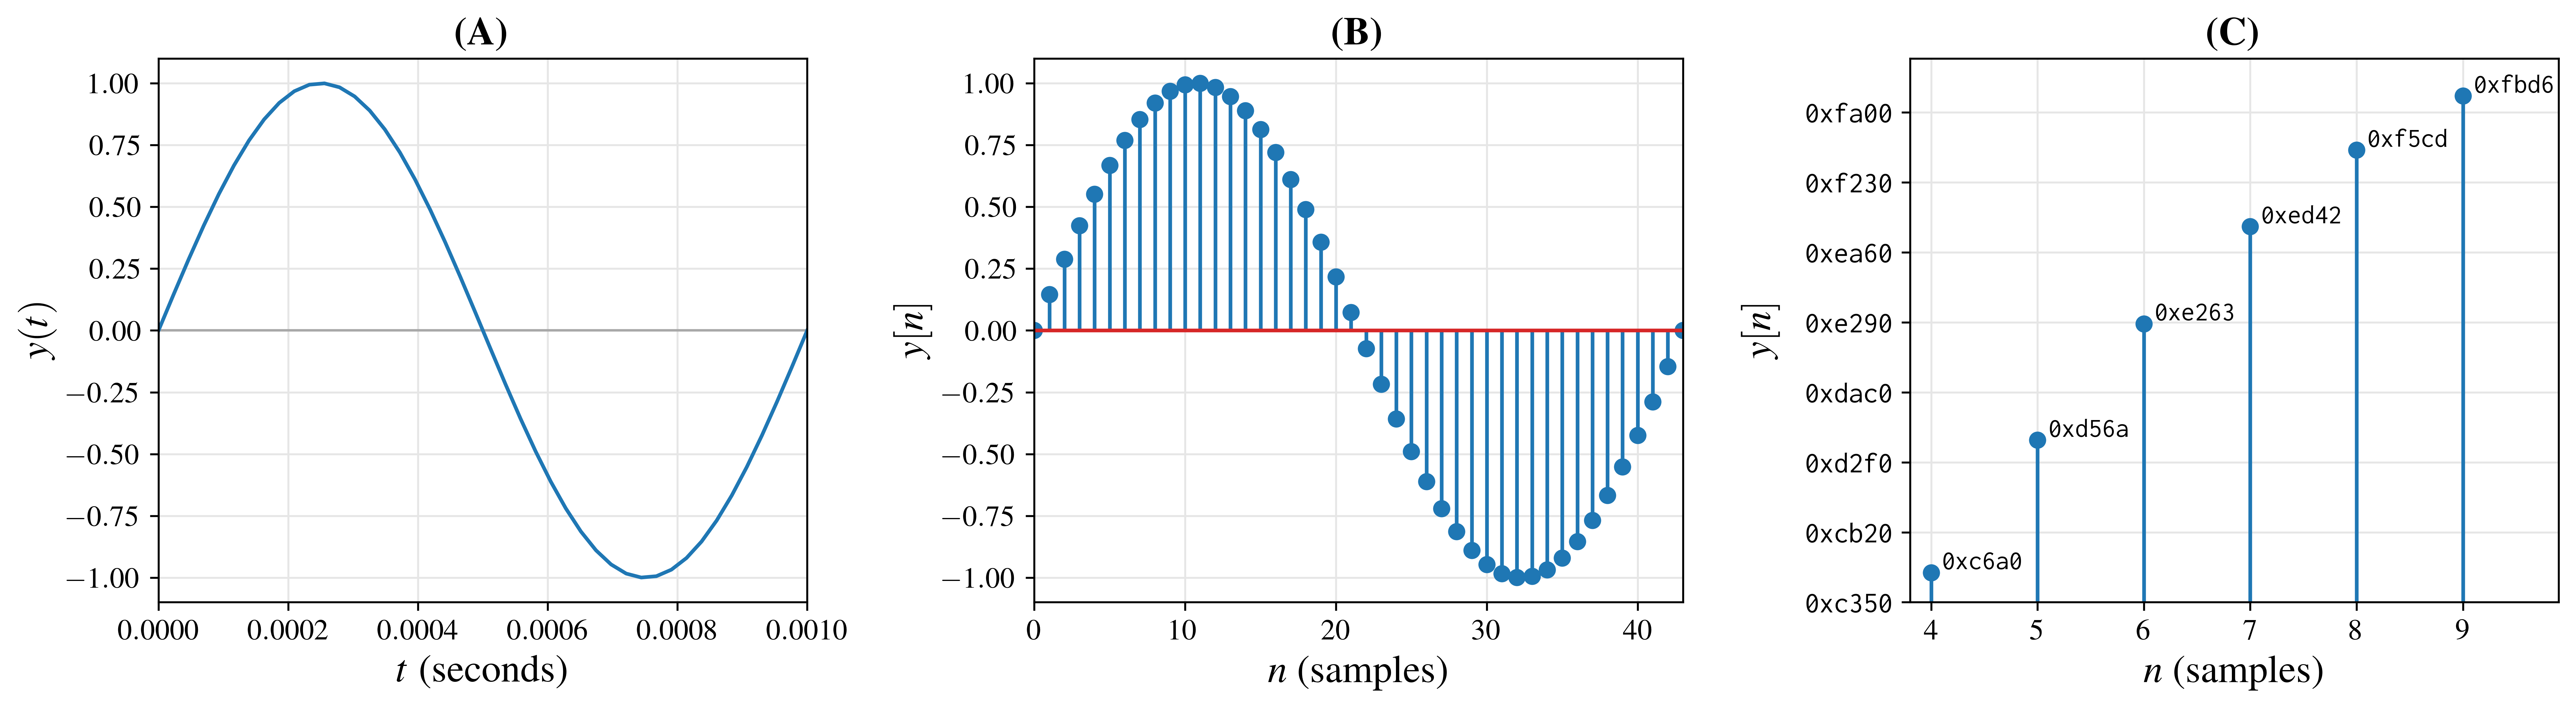
\includegraphics[width=\textwidth]{figures/digital-signal}
    \caption{
        An audio signal (\qty{1}{\kHz} sine wave);
        (a) in continuous time;
        (b) sampled at intervals of $1/Fs$ seconds, with $F_s=~$\qty{44.1}{\kHz};
        (c) detail of (b) with sample amplitudes converted to 16-bit hexadecimal
        values.
    }
    \label{fig:signal-samples}
\end{figure}

Samples undergo format conversion at various stages during processing, such as
from an integer pulse code modulation (PCM) filetype to a stream of floating
point audio samples in a digital audio workstation (DAW), or from a floating
point audio stream in an audio device driver to an integer stream to be handled
by a hardware codec.
For the most part, the user, and even the developer of audio software, need not
concern themselves with the rudiments of sample representation and conversion;
as shall be shown, however, under certain circumstances these fundamental
aspects of digital audio systems must be dealt with directly.

\subsection{Numerical Representation}\label{subsec:numerical-representation}

Digital audio samples are ultimately described as streams of binary numbers.
Broadly speaking, the more binary digits (\textit{bits}) available for each
sample, the greater the resolution in terms of distinct amplitudes that can be
represented, with ramifications for dynamic range and signal-to-noise ratio, as
well as for storage and throughput.
Integer sample formats, such as commonly-encountered 16 and 24-bit, offer
comparatively poor resolution at low amplitudes due to the incongruity between
the linear distribution of their values versus the logarithmic nature of sound
intensity.
Floating point formats, by contrast, feature a logarithmic distribution of
available values; the IEEE standard for single-precision (i.e.\ 32-bit) floating
point numbers~\citep{ieee_ieee_1985} describes numbers over the interval
$\pm[0,\num{3.403e38}]$ but with precision clustered around zero, around half
the available values lying in the interval $[-1, 1]$.

To give a brief example, consider the 16-bit case, and a single 16-bit integer
audio sample:
\begin{equation*}
    \texttt{11010101 01101010}
\end{equation*}
Separating the bits into two groups of eight is reflective of the fact that the
eight-bit \textit{byte} is typically the unit of transmission in computer
systems.
Grouping the bits in this way points to their expression in hexadecimal format,
transforming the bytes into more easily-digestible morsels of two digits apiece:
\begin{equation*}
    \texttt{d5 6a}
\end{equation*}
A number of this kind may also be seen represented (in C and C++ code for
example) as \texttt{0xd56a}, with `\texttt{0x}' indicating that the number to
follow is in base sixteen.
Sixteen bits grant access to $2^{16}=\num{65536}$ distinct amplitude values for
each sample; what the above tells us is that, in decimal terms, this sample
should take the \num{54634}\textsuperscript{th} amplitude value\footnote{
    For convenience and explicitness elsewhere in the text, decimal equivalents
    to hexadecimal numbers will be indicated with subscript 10, e.g.
    \numDec{54634}.
}.

\subsection{Storage and Transmission}\label{subsec:storage-and-transmission}

The above binary and hexadecimal representations hint at the property of
\textit{endianness}, i.e.\ the order in which a number's component bits and
bytes appear~\citep{cohen_holy_1981}.
The given examples mirror the left-to-right nature of western written language
and numbers, being \textit{big endian} at the levels of both bit and byte, with
the \textit{most significant bit} (and \textit{most significant byte}, both
abbreviated \textit{MSB}) appearing first.

To paraphrase Cohen~\citep{cohen_holy_1981}, if the unit of digital audio
transmission was \textit{an audio signal}, then endianness would not be a
matter of concern.
Practically speaking, however, to be handled by software or hardware, or
transmitted over a network, audio signals must be decomposed into a hierarchy
of temporally-distributed blocks, those blocks into samples, samples into bytes,
and bytes into bits;
correct endianness must be observed with respect to differing computer
architectures, file formats, and transmission protocols.

The PCM WAV file format, for example, dictates that the least significant byte
of each sample is stored first \textemdash{} little endian \textemdash{} but
that bit order should be big endian~\citep{noauthor_multimedia_1991};
thus the hexadecimal number above should be stored in a \texttt{.wav} file as
\texttt{6ad5}.
The ethernet standard for communication over local area computer
networks~\citep{noauthor_ieee_2018}, by contrast, calls for something akin to
the opposite:
the most significant byte is transmitted first, with each byte sent
little-endian;
returning to the binary representation:
\begin{equation*}
    \texttt{11010101 01101010} \quad\rightarrow\quad \texttt{10101011 01010110}
\end{equation*}
Note, however, that network packet capture software such as
Wireshark\footnote{\url{https://www.wireshark.org/}} reports the bytes of
intercepted packets with most significant bit first.

    \section{Networked Audio}\label{sec:networked-audio}

\todo[inline]{Less detail on telephony?}
The transmission of audio data has been a topic of research interest since the
earliest days of computer networking as it is recognised today, i.e.\ over
packet-switched networks, whereby data to be transmitted is grouped into
packets, each consisting of a header and a payload.
Voice transmission over ARPANET was being conducted as early as
1974~\citep{schulzrinne_voice_1992} and the first standard for voice
communication over packet-switched networks \textemdash{} the Network Voice
Protocol (NVP) \textemdash{} was released in
1977~\citep{cohen_specifications_1977}.

With its references to `calling' and `ringing', it is clear that the NVP
standard was intended for digital telephony.
Indeed, research on networked audio was primarily concerned with telephony well
into the 1990s, focusing on real-time voice communication over wide area
networks (WAN) with efforts centring on \textit{quality of service} (QoS),
particularly with regard to the perennial issues of latency, packet loss, and
network jitter \textemdash{} inconsistencies in the rate of packet
transmission~\citep{hardman_reliable_1995,hardman_successful_1998}.
Work at this time dealt with streams of compressed audio data, and speech
coding algorithms to overcome the deleterious effects of dropped packets over
unreliable network paths and low-bandwidth connections.

Whereas the priority for digital telephony, and later voice over IP (VoIP)
systems, is intelligibility, for musical purposes fidelity, and the use of
uncompressed audio signals, is of greater concern.
With the increasing availability of high-speed internet connections in the late
1990s came research into transmitting uncompressed audio data over the
internet~\citep{chafe_simplified_2000,xu_real-time_2000}.
Work of this sort was spearheaded by the \textit{SoundWIRE} project, developed
by researchers at McGill University and the Centre for Computer Research in
Music and Acoustics (CCRMA) at Stanford University, and took the form of
a wide variety of experiments with high quality audio over both WAN and local
area networks (LAN).
These experiments included LAN-based real-time musical
performances~\citep{chafe_simplified_2000}, concert streaming over
WAN~\citep{xu_real-time_2000,chafe_simplified_2000}, and sonification of QoS via
a distributed digital waveguide dubbed the
\textit{Network Harp}~\citep{chafe_simplified_2000,chafe_physical_2002}

\subsection{Protocols and Systems}\label{subsec:protocols-and-systems}

VoIP research in the 1990s focused on matters such as audio codecs and data
compression~\citep{turletti_inria_1995,hardman_successful_1998}, seeking a
compromise with the \textit{best-effort} nature of internet service.
The SoundWIRE project, in search of high audio quality, turned its attention
directly to the basic transport layer protocols of the Internet Protocol suite:
Transmission Control Protocol (TCP) and User Datagram Protocol (UDP).
Chafe et al.\ characterised their compression-free system as taking a
``simplified approach''~\citep{chafe_simplified_2000} to networked audio,
emphasising the importance of delivering multichannel audio of at least CD
quality (16-bit, \qty{44.1}{\kHz}) with as little latency as possible.

SoundWIRE experiments included using TCP for unidirectional transmission such as
concert streaming.
TCP is in fact a bidirectional protocol, but its \textit{connection-oriented},
one-to-one design, whereby networked entities establish a connection via a
`handshake', following which packets of data are exchanged, allows for
mechanisms that guarantee packet ordering and provide protections against packet
loss~\citep{schiavoni_alternatives_2013,al-dhief_performance_2018}.
These mechanisms mean that, at the expense of increased latency, quality of
service, and thus audio fidelity, is ensured; ideal for a remote concert
scenario.
%The strict one-to-one nature of TCP clearly places limits on its
%applicability to distributed computing, however.

UDP by comparison is a \textit{connectionless} protocol, providing no guarantees
regarding the integrity of the stream of network data, but equally none of the
computational, or indeed temporal, overhead that such guarantees introduce.
A network entity can send UDP packets to a network address irrespective of
the presence or otherwise of an entity at that address.
Further, \textit{many-to-many} (multicast) and \textit{one-to-many} (broadcast)
modes of transmission are possible via address spaces reserved as part of the
internet protocol standard~\citep{meyer_iana_2010}.
Via UDP, SoundWIRE was able to run as a distributed digital waveguide over a
WAN spanning around \qty{4500}{\km}~\citep{chafe_simplified_2000}.

From the SoundWIRE project emerged
\textit{JackTrip}~\citep{caceres_jacktrip_2010,caceras_jacktripsoundwire_2010},
a hybrid system that couples a TCP handshake with audio transmission over UDP,
thus sidestepping the overhead of TCP packet flow control.
Rather than relying on TCP's built-in mechanisms for stream integrity, JackTrip
supplements UDP with a number of optional buffering strategies that aim to
tailor its use to operation over local versus wide area networks.
In this sense it is more flexible than TCP, but in effect JackTrip moulds UDP
transmission into something akin to the connection-oriented model of TCP, and,
in its `hub server' mode, into a kind of \textit{multiple one-to-one} design
\textemdash{} multicast transmission is not possible.

UDP has emerged as the protocol of choice for platforms enabling remote musical
collaboration, serving as the basis for systems such as
NetJACK~\citep{carot_netjack_2009}, part of the JACK Audio Connection Kit (a
cross-platform audio host), Jamulus~\citep{fischer_case_2015},
Soundjack~\citep{renaud_networked_2012}, and other jamming-focused platforms,
plus more recent entrants such as the closed-source, but ultimately UDP-based
Elk OS~\citep{turchet_elk_2021}.
UDP even plays a fundamental role in proprietary systems such as Dante (Digital
Audio Network Through Ethernet)~\citep{noauthor_what_nodate}.

\subsubsection{AoE in the Audio Industry}

In parallel with the work being carried out by researchers such as those
developing SoundWIRE, JackTrip and NetJACK, audio industry bodies were taking
an interest in networked audio.
Prominent amongst these bodies were the IEEE (Institute of Electrical and
Electronics Engineers) and AES (Audio Engineering Society) standards groups,
and companies like Audinate, the creators of the Dante system.
Traditional large-scale audio systems such as those used in broadcast, concert
venues and recording studios rely on the installation of unwieldy systems of
analogue hardware and cabling, with many potential points of failure.
Seeking literally to lighten the load posed by ``hundreds of
kilograms''~\citep{bakker_introduction_2014} of analogue cabling in analogue
audio installations, in the 2000s industry entities were looking to high speed
ethernet as a means to simplify the provision of high-quality, multichannel
audio in industry settings.

Dante, with its promise of low-latency, highly-multichannel audio over ethernet,
and device synchronisation via Precision Time Protocol (PTP), has become the de
facto standard in this area~\citep{bakker_introduction_2014}.
In 2011, IEEE released the Audio Video Bridging (AVB, IEEE 802.1) standard,
and AES67 followed in 2013; these open technical standards describe operation
at layers below TCP and UDP in the OSI (Open Systems Interconnection)
model~\citep{}\todo[inline]{Add source for OSI}, and provide frameworks for
interoperability between AoE and AoIP systems, including mechanisms for device
discovery and synchronisation, again via PTP\@.
Being standards, and not implementations in themselves, it is then up to
manufacturers to implement the appropriate recommendations in their products.
(AES67, for example, has in fact been implemented in Dante.)

Bakker et al.\ refer to Dante as an ``open'' system.
This is perhaps true in the sense that companies can incorporate the Dante
system into their own products under licence from Audinate, but, from the
perspective of the academic community, Dante is very much a closed-source
initiative and not a suitable platform for research.
Open implementations of AVB and AES67 could be of interest, however their
reliance on PTP, support for which is not offered by ubiquitous, low-cost
networking equipment, raises the barrier to entry to systems based on these
standards.
Ultimately, if an accessible solution is sought, attention must be turned back
to the transport layer, and UDP\@.

\subsection{Anatomy of a Datagram}\label{subsec:anatomy-of-a-datagram}

\begin{figure}[h]
    \centering
    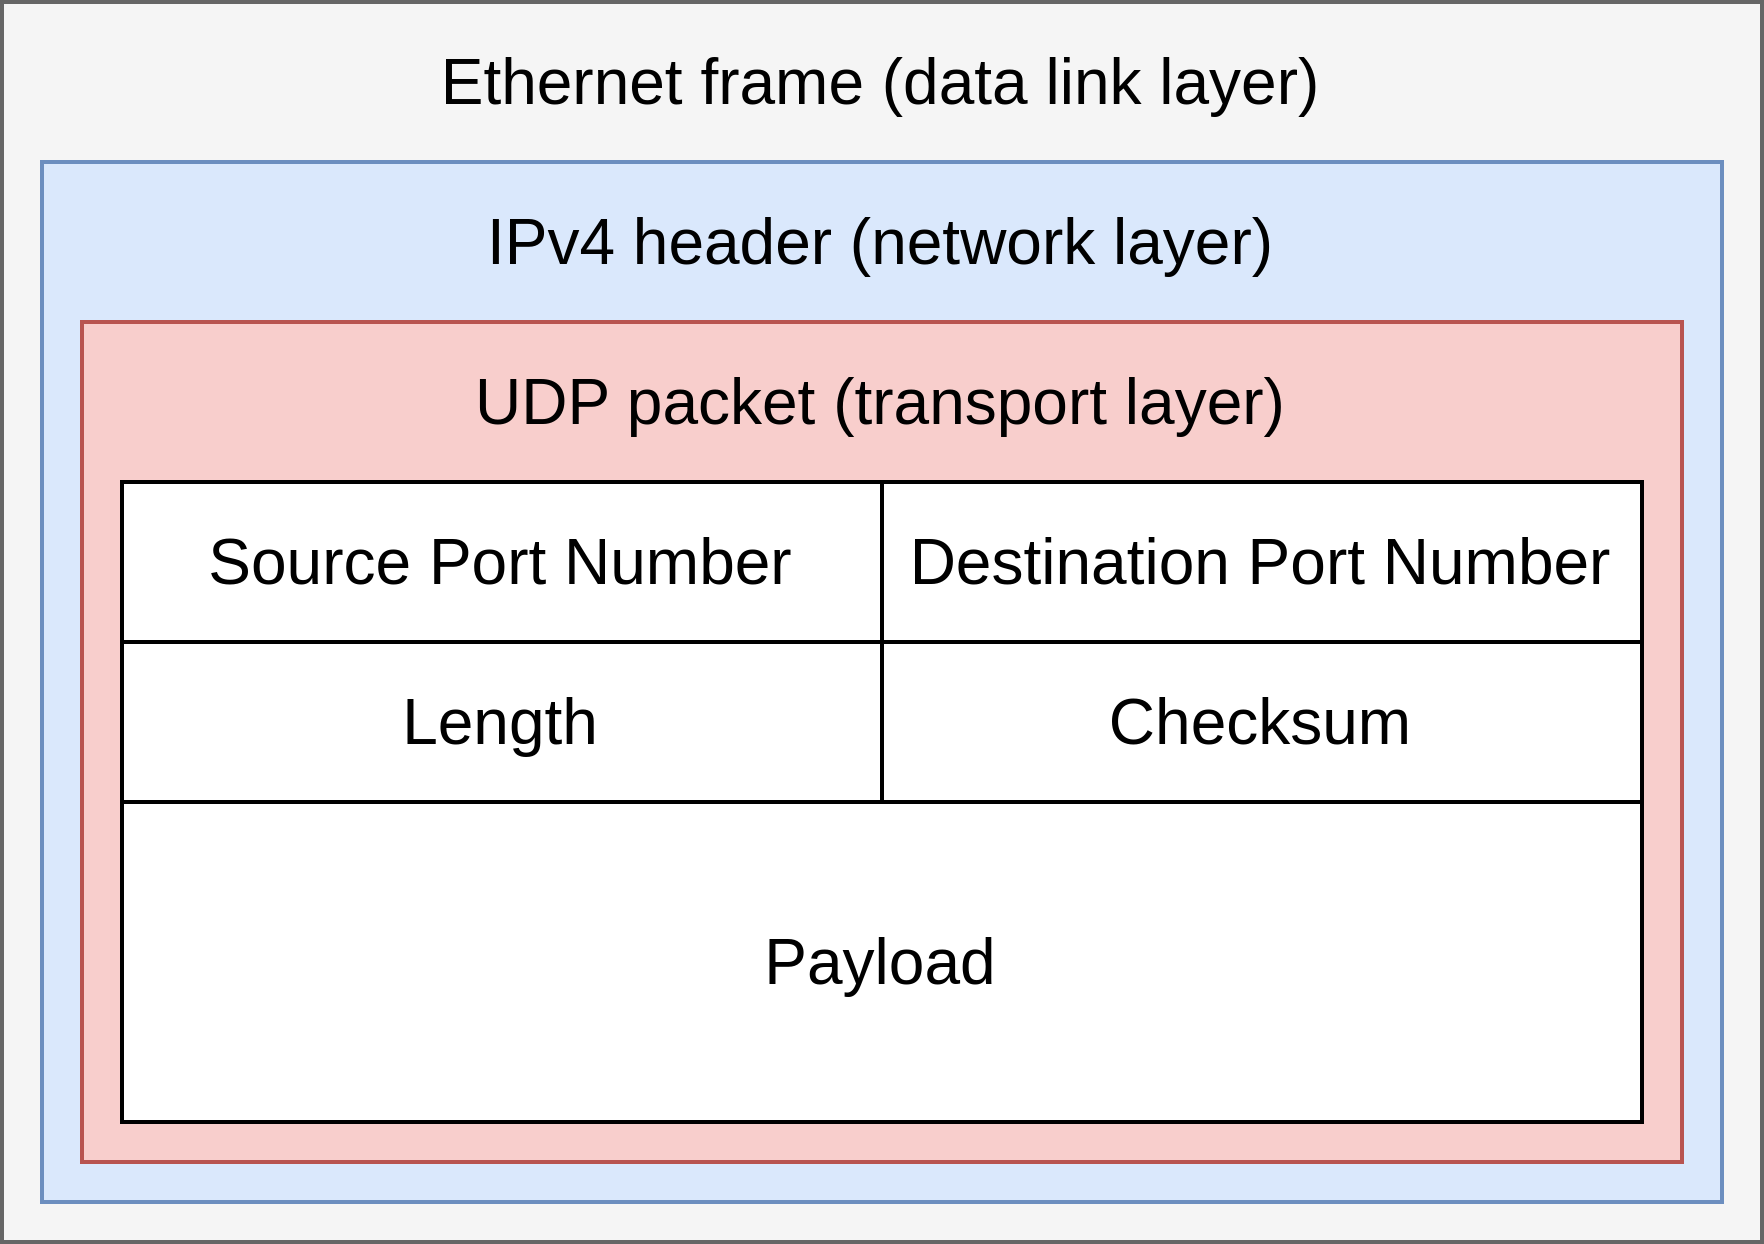
\includegraphics[width=.5\textwidth]{figures/udp}
    \caption{Structure of an ethernet frame containing a UDP packet.}
    \label{fig:udp-frame}
\end{figure}

A UDP packet consists of data encoded in 8-bit integer format.
Being a transport layer protocol, a UDP packet is in fact preceded in an
ethernet frame by information relating to lower layers in the OSI hierarchy: the
network layer and the data link layer.
The structure of a UDP packet (within an ethernet frame) is shown in
\figref{fig:udp-frame}.

\codeinputlisting[float=h]
{text}
{listings/udp-packet.txt}
{Network capture: ethernet frame containing a UDP packet}
{packet-hello-world}
\noindent
The ethernet frame in listing~\ref{listing:packet-hello-world} was generated
using the Netcat (\texttt{nc}) command line utility\footnote{
    \url{https://nc110.sourceforge.io/}
}, and captured with Wireshark network traffic analysis software.
Four-digit numbers to the left indicate the hexadecimal index of the byte
at the beginning of the corresponding line.
The central block of two-digit hexadecimal numbers are a representation of the
bytes in the ethernet frame, labelled above by byte position.
The block of characters to the right are the same data encoded as ASCII
characters.

\begin{table}[h]
    \centering
    \begin{tabular}[h]{c c c c}
        Start           & End             & Purpose                 & Value                                        \\
        \midrule[1pt]
        \texttt{0x0000} & \texttt{0x000d} & Ethernet header         &                                              \\
        \midrule
        \texttt{0x0000} & \texttt{0x0005} & Destination MAC address &                                              \\
        \texttt{0x0006} & \texttt{0x000b} & Source MAC address      &                                              \\
        \texttt{0x000c} & \texttt{0x000d} & Ethernet frame type     & \texttt{0x0800}: IPv4                        \\
        \midrule[1pt]
        \texttt{0x000e} & \texttt{0x0021} & IPv4 header             &                                              \\
        \midrule
        \texttt{0x0017} & \texttt{0x0017} & Protocol                & \texttt{0x11}: UDP                           \\
        \texttt{0x001a} & \texttt{0x001d} & Source IP address       & \texttt{0xac1efedf}: \texttt{172.30.254.223} \\
        \texttt{0x001e} & \texttt{0x0021} & Destination IP address  & \texttt{0x7f000001}: \texttt{127.0.0.1}      \\
        \midrule[1pt]
        \texttt{0x0022} & \texttt{0x0029} & UDP header              &                                              \\
        \midrule
        \texttt{0x0022} & \texttt{0x0023} & Source port number      & \texttt{0xed3f}: \numDec{60735}              \\
        \texttt{0x0024} & \texttt{0x0025} & Destination port number & \texttt{0x22b8}: \numDec{8888}               \\
        \texttt{0x0026} & \texttt{0x0027} & Length                  & \texttt{0x0016}: \numDec{22}                 \\
        \midrule[1pt]
        \texttt{0x002a} & \texttt{0x0037} & UDP Payload             &                                              \\
        \bottomrule
    \end{tabular}
    \label{tab:packet-structure}
    \caption{Description of selected fields in the UDP packet depicted in
    listing~\ref{listing:packet-hello-world}.}
\end{table}

Bytes \texttt{0x0000} to \texttt{0x000d} make up the ethernet header,
consisting of the media access control (MAC) addresses of the destination and
source; the final two bytes of the ethernet header, \texttt{0x0800}, indicate
that this is an \textit{internet protocol version 4} frame.
Bytes \texttt{0x000e} to \texttt{0x0021} are the IPv4 header; this contains
information about the internet protocol part of the packet, such as its length
in bytes \textemdash{} \texttt{0x002a} (\numDec{42}) \textemdash{} and
the source and destination IP addresses, encoded as groups of four-bytes.
The source IP address, for example, is \texttt{0xac1efedf}, a 32-bit encoding
of the more familiar-looking \texttt{172.30.254.223}.

Beginning at byte \texttt{0x0022} is the UPD header.
This contains the source port (\texttt{0xed3f}, \numDec{60735}), destination
port (\texttt{0x22b8}, \numDec{8888}), the length of the UDP part of the frame
(\texttt{0x0016}, \numDec{22} bytes) and ends with a checksum, which
can be used to verify the integrity of the packet\footnote{
    In the remainder of this work it is assumed that transmission over LAN is
    unlikely to result in packet corruption; the UDP checksum is not used.
}.
The packet payload begins at byte \texttt{0x002a}, and consists of bytes
corresponding with the ASCII characters \texttt{Hello, world!}, plus
\texttt{0x0a}, the line feed (LF) character, captured and sent by Netcat when
the user hit the return key.

Netcat takes data supplied to a computer's standard input stream, in this
case characters supplied to a terminal emulator, and uses this data as the
payload for the packet to be transmitted.
The payload of a UDP packet can of course consist of any data which can be
appropriately byte-encoded, such as a stream of audio samples, or audio control
data such as MIDI or OSC messages.

Ethernet frames, and UDP datagrams by extension, are subject to size
limitations.
The maximum transmissible unit (MTU) of a transport medium is the limit on the
size of a packet that can be sent without fragmentation, i.e.\ without being
split into multiple sub-packets.
Two bytes (sixteen bits) are allocated to the `Total Length' field of the IPv4
header, which suggests an MTU of $2^{16}-1=~$\num{65535} bytes;
in practice, however, the data link layer imposes a basic limit of \num{1500}
bytes on the payload of an ethernet
frame~\citep{schiavoni_alternatives_2013,noauthor_ieee_2018}.

\subsection{Hardware Platforms}\label{subsec:hardware-platforms}

\todo[inline]{Move hardware elsewhere}
\dots

Recent years have seen the emergence of a number of small, low-cost, open-source
platforms for embedded development, perhaps best known amongst these being
Arduino\footnote{\url{https://arduino.cc/}}.
Though support for audio is limited via official Arduino models, a number of
audio-specific, Arduino-like systems have been produced, such as various
ESP32\footnote{\url{https://espressif.com/en/products/devkits/esp-audio-devkits}}
and STM32\footnote{\url{}} models, Daisy Seed\footnote{\url{}} (itself an STM32-based board), and the Teensy family of microcontroller
development boards\footnote{\url{https://pjrc.com/store/teensy41.html}}.

    \section{Audio Spatialisation}\label{sec:audio-spatialisation}

Audio spatialisation is, plainly enough, the practice of distributing sound in
space.
In terms of the reproduction of \textit{primary sound sources}, i.e.\ sound
captured by microphones, recorded as digital audio files, or synthesised in
real-time, spatialisation can be achieved simply by delivering those primary
sources to \textit{secondary sound sources}, i.e.\ loudspeakers, placed at
arbitrary positions relative to a listener.
Such an approach is, of course, inflexible;
loudspeakers being stationary entities by-and-large, the idea of moving a sound
source is physically impractical, and, that of locating a sound source
between loudspeaker positions physically impossible.
Taking advantage of auditory cues, however, and the nature of the propagation
of sound, it is possible to suggest the presence of primary sources at
arbitrary locations, independent of the secondary source distribution.
The motivation behind audio spatialisation, then, is to create (or indeed
\textit{recreate}) sonic environments for creative and immersive purposes, such
as for virtual reality experiences, in cinematic settings, for music production
or art installations, to give but a handful of examples.

A number of techniques exist for what is termed \textit{sound field
synthesis}~\citep{ahrens_analytic_2012,nicol_sound_2017}, all of which
essentially take the form of applying some manner of \textit{driving function}
to an input audio signal to generate an appropriate driving signal to be
delivered to a secondary sound source in the listening
environment~\citep{ahrens_analytic_2012}.
For a loudspeaker at position $\mathbf{x} = \begin{bmatrix}
                                                x & y & z
\end{bmatrix}^T$, the driving signal $\hat{D}(\mathbf{x}, \omega)$ can be
expressed, in the frequency domain, as the product of the input signal,
$\Sigin(\omega)$ and the driving function $D(\mathbf{x}, \omega)$:
\begin{equation}
    \label{eq:driving-signal-freq}
    \hat{D}(\mathbf{x},\omega) = \Sigin(\omega) \cdot D(\mathbf{x},\omega),
\end{equation}
where $\omega$ denotes radian frequency, $\omega = 2\pi f$, and $f$, in turn,
is time frequency.
Moving to the time domain, the multiplication of the input signal and driving
function changes to a convolution, and equation~\eqref{eq:driving-signal-freq}
becomes:
\begin{equation}
    \label{eq:driving-signal-time}
    \hat{d}(\mathbf{x},t) = \sigin(t) \ast d(\mathbf{x},t),
\end{equation}
where $t$ denotes time.

An early sound field synthesis approach, referred to as an `acoustic
curtain'~\citep{ziemer_wave_2020} entailed placing microphones in one space,
such as a concert auditorium, and, in another space, loudspeakers at locations
corresponding to those of the microphones.
In this case, there are as many input signals $\hat{S}_k(\omega)$ as there are
microphones, and the driving function reduces to a `pass-through' of each
signal to its corresponding loudspeaker, i.e. $D_k(\mathbf{x}, \omega) = 1$.

The acoustic curtain is a relatively rarely-deployed technique (though similar
recreation of `real' sound fields is still conducted, albeit typically by way
of ambisonic recording and reproduction) and sound field synthesis is most
often concerned with the distribution and movement of artificial or arbitrary
sound sources.
Commonly-employed approaches to sound field creation can be grouped into two
broad categories: amplitude- and time-based panning techniques, and physical
sound field recreation approaches.

\subsection{Periphony}\label{subsec:periphony}

The former, \textit{periphonic}, types are perhaps more familiar to the
layperson and encompass stereophony and surround-sound systems, consisting of
secondary sources in a horizontal planar arrangement equidistant to the
listening position.
These techniques exploit the interaural level difference (ILD) cue, i.e.\ the
difference in perceived amplitude relative to the listener's
ears~\citep{pulkki_virtual_1997,verheijen_sound_1998,ziemer_wave_2020}, to
encourage the listener to localise sound to a position on the circumference of
an arc or circle around the listening position.
This is achieved by weighting the amplitudes of signals sent to the
secondary sources, creating a ``phantom'' sound source that may appear to
emanate from a position between loudspeakers.
For systems of this sort, the driving function is a constant scalar value, or,
for a moving phantom source, a time-varying function that returns a scalar
value.
Such periphonic approaches can extend to three dimensions in the case of
vector base amplitude panning (VBAP)~\citep{pulkki_virtual_1997}, which uses
trios of speakers to position phantom sources on the surface of a sphere
with the listening position at its origin.

Time-based panning effects, by contrast, make use of the interaural time
difference (ITD) cue to give the impression of a phantom source located toward
the loudspeaker producing the signal at the earliest
time~\citep{pulkki_virtual_1997,verheijen_sound_1998}.
Thus the driving function for a time-based panning system is a delay of the
form:
\begin{equation}
    d(\mathbf{x},t) = \delta(t - \tau),
    \label{eq:time-driving-function}
\end{equation}
where $\tau$ is the duration of the delay.

The effects of ILD and ITD cues may transfer to headphone-based listening,
in which case, rather than periphonic, they become a sort of \textit{in-head}
localisation~\citep{ahrens_analytic_2012}.
It is worth mentioning that these cues vary in their effectiveness with
frequency and, excepting the case of headphone-based listening, intersect with
cues related to listener's torso~\citep{verheijen_sound_1998} and the
head-related transfer
function~\citep{de_poli_physically_1998,geier_object-based_2010}.

Periphonic approaches (again, headphones excepted) are subject to the
phenomenon of an ideal listening position, or
\textit{sweet-spot}~\citep{verheijen_sound_1998,nicol_sound_2017}, that is a
listening position away from which the spatialisation effect is significantly
degraded.
As such, these techniques are not suited to subjection to multiple listeners,
nor to immersive auditory experiences permitting the participant to move freely
about their environment.
Additionally, phantom sources are inherently bound to the periphery on which
they reside;
there is no authentic way to model a phantom source at greater (or lesser)
distance, though using reverberation and amplitude cues may offer a satisfactory
perceptual impression.

\subsection{Physically-Inspired Techniques}

\begin{figure}[ht]
    \centering
    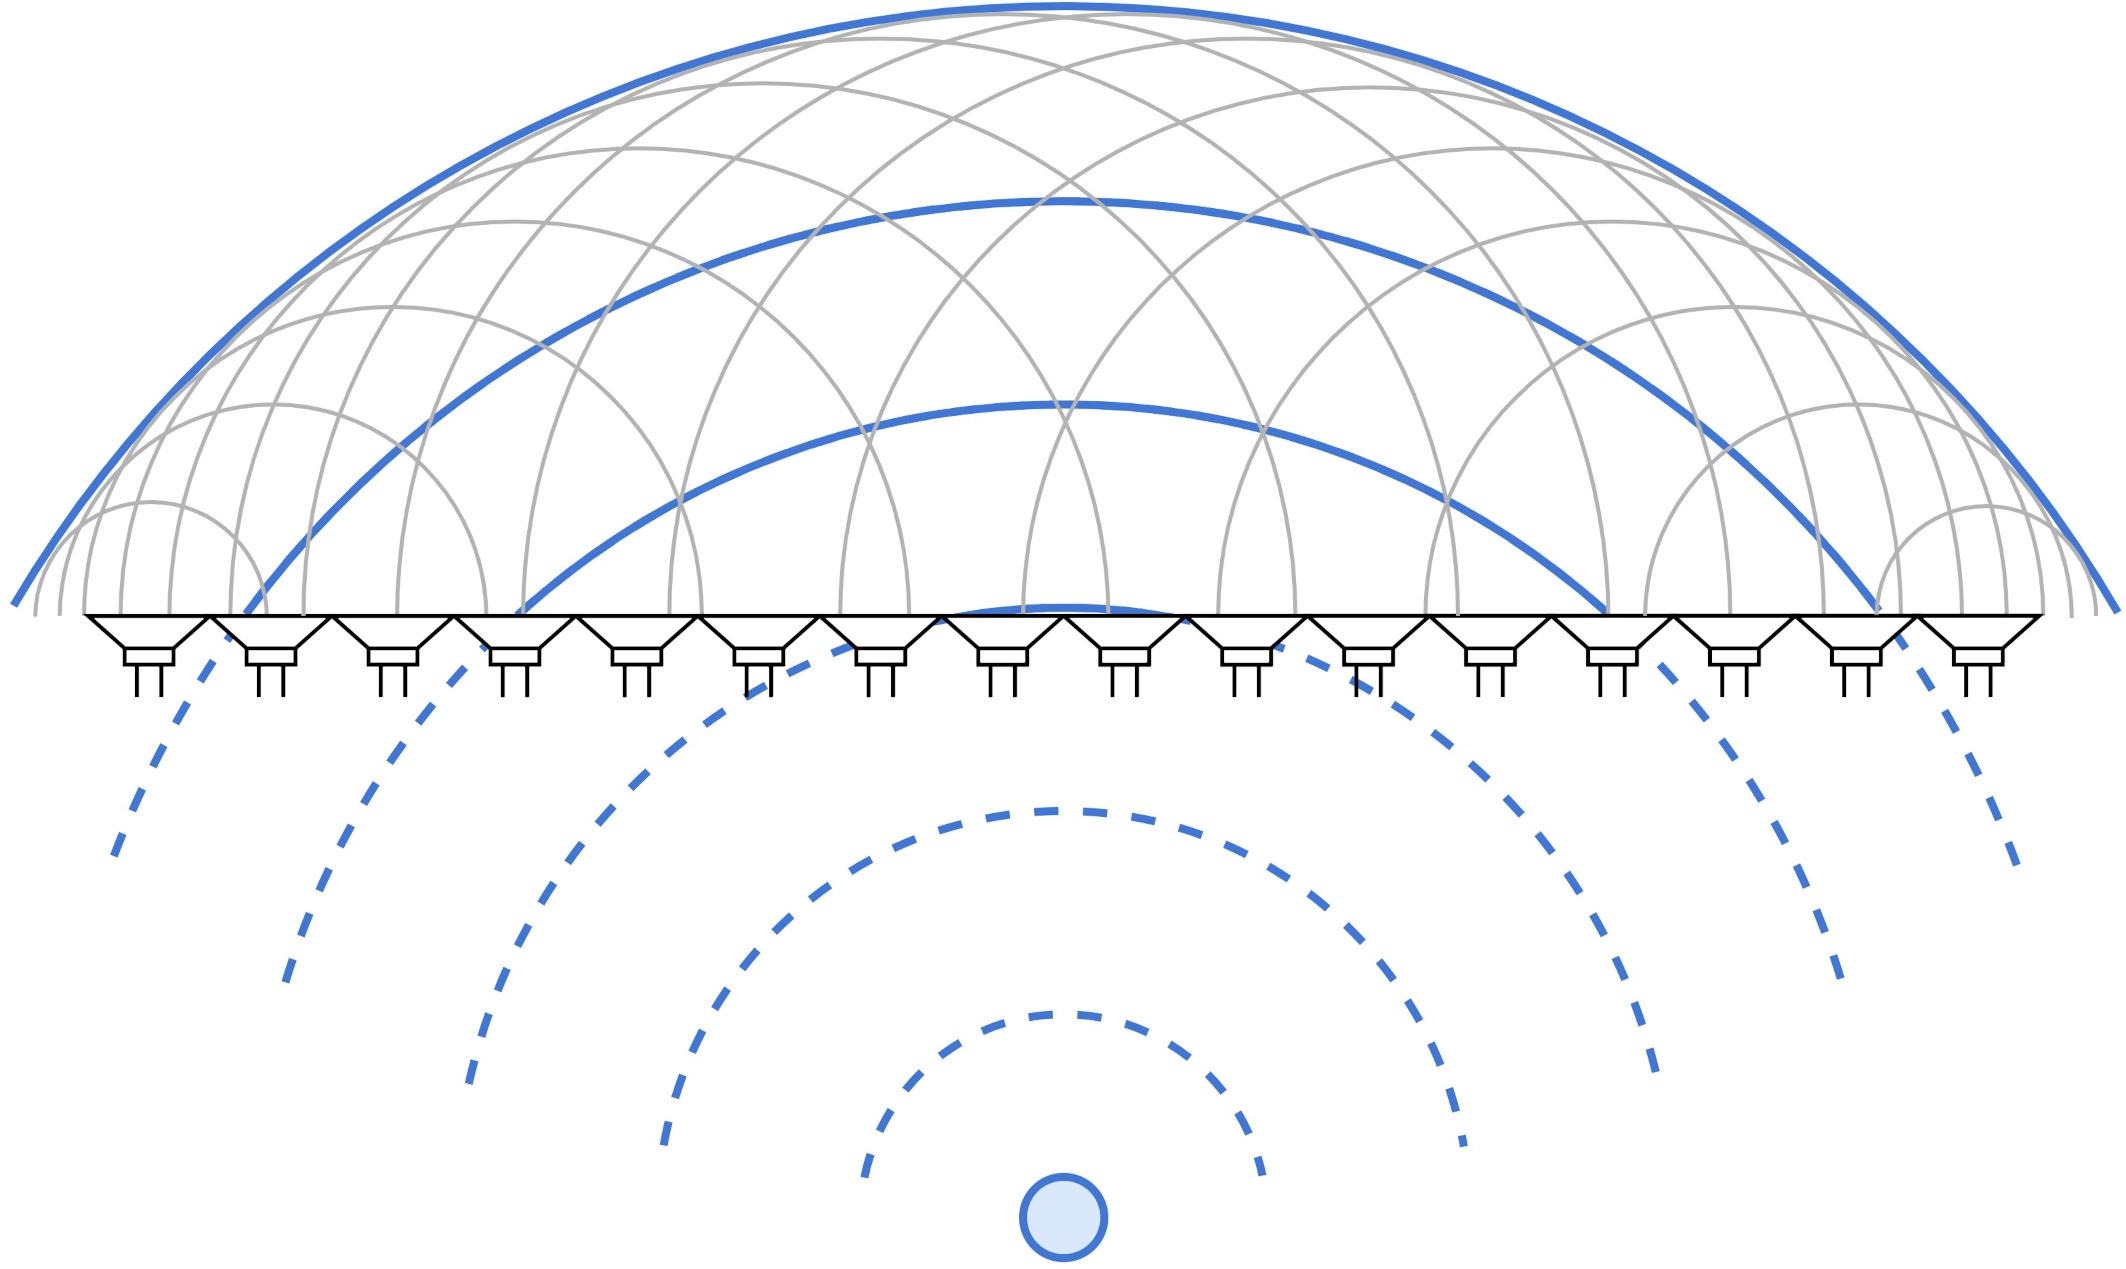
\includegraphics[width=\textwidth]{figures/wfs_1}
    \caption{\textit{Holophony}.
    Huygens' principle states that the propagation of a wavefront
    can be recreated by a collection of secondary point sources.
    The bottom of the figure represents a virtual sound field, and the top a
    real sound field, separated by a row of secondary point sources
        (loudspeakers).
        The small blue circle represents a virtual sound source and the blue
        dashed arcs are virtual wavefronts associated with that sound source;
        the grey arcs are wavefronts produced by the array of secondary point
        sources;
        the solid blue arcs represent the propagation of a reconstructed
        wavefront in the real sound field.}
    \label{fig:wfs_1}
\end{figure}

Physical approaches fall into two main types: wave field synthesis (WFS) and
ambisonics (and higher-order ambisonics \textemdash{} HOA). Rather than
directly manipulating sound localisation cues, these types seek to trigger
those cues indirectly by synthesising a sound field as if it had been created
by `true' acoustic sources, as opposed to loudspeakers.
In the case of ambisonics, the sound field is decomposed into `spherical
harmonics', spatial functions described by linear sums of directional
components of increasing order~\citep{nicol_sound_2017}.
Spherical and plane waves can be reproduced, corresponding with virtual
point sources and sources at `infinite distance' respectively.

Ambisonics, like periphonic approaches, suffers from a sweet-spot effect which
worsens with attempts to reproduce sounds of higher frequency.
The ideal listening area can be broadened by implementing ambisonics at higher
order, increasing the density of the distribution of secondary sources.
Doing so obviously has ramifications for the physical complexity of an
ambisonics installation, and, since higher-order spherical modes must be
calculated, in terms of computational demands placed on the system.

\subsubsection{Wave Field Synthesis}

Reminiscent of the acoustic curtain, WFS is based upon Huygens' principle,
originating in the field of optics, which states that a propagating
wavefront can be recreated by a distribution of secondary point
sources~\citep{mueller_acoustic_1971,berkhout_acoustic_1993,
    belloch_performance_2021}(see \figref{fig:wfs_1}).
It is variously termed a form of \textit{acoustic holography} or
\textit{holophony}~\citep{berkhout_holographic_1988,ahrens_analytic_2012}.
Effectively, by timing the reproduction of an input signal at an array of
secondary sources, a wavefront associated with a virtual sound source can be
synthesised.
To simulate distance cues, a filter can be applied to model losses to the
virtual medium of acoustic propagation.
The principle assumes a continuous array of secondary sources but of course in
practice it is necessary to use a discrete array of loudspeakers, which,
much as is the case with HOA, has ramifications for spatial resolution;
to mitigate the issue of spatial aliasing, whereby sounds of higher frequency
cannot be recreated unambiguously~\citep{winter_geometric_2018},
secondary sources should be placed very close together.
Consequently, to serve a large listening area, many speakers, and thus many
audio channels, are required.

Via appropriate timing of the delivery of a primary sound source to the
secondary source array, it is possible to synthesise virtual sound sources,
plane waves, and \textit{focused} sound sources, corresponding with concave,
flat, and convex synthesised wavefronts respectively; the latter, dependent
on the location of the listener, appear to emanate from within the real
sound field, rather than its virtual counterpart.

\begin{figure}[ht]
    \centering
    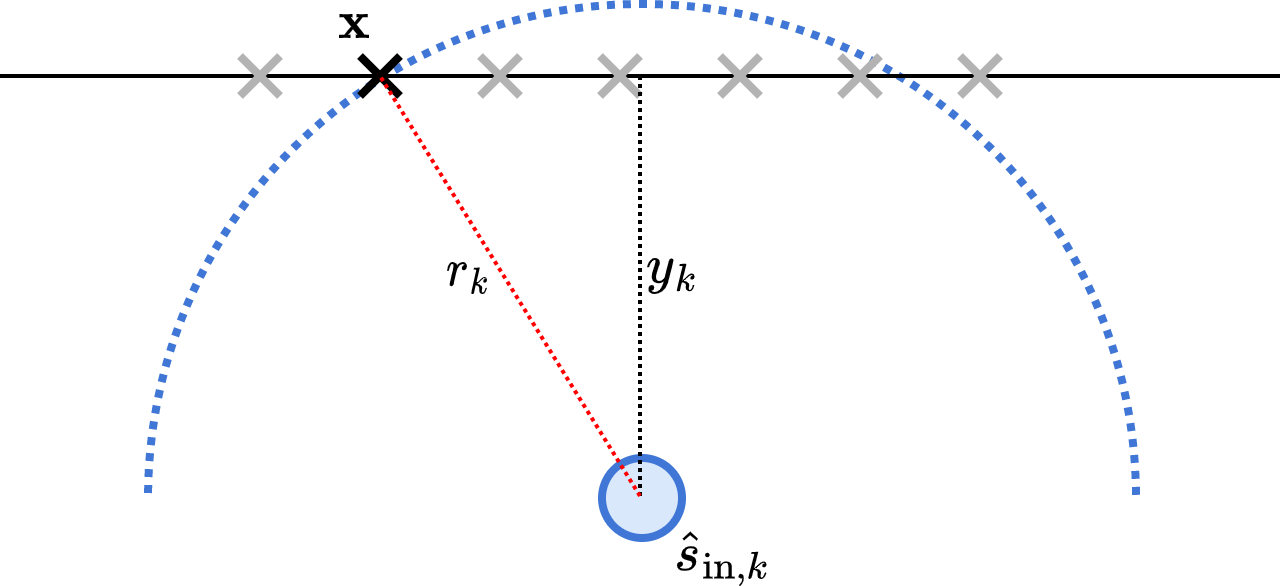
\includegraphics[width=.75\textwidth]{figures/wfs_2}
    \caption{
        The driving signal for the WFS secondary source at position $\bfx$,
        for virtual primary source $\sigink$, is dependent on the distance
        $r_k$ of the primary source from the secondary source.
        This corresponds with a propagation delay via the simulated medium of
        propagation, coupled with a filter describing losses to that medium.
    }
    \label{fig:wfs_2}
\end{figure}

Focusing on the former kind, however, for $m$ virtual sources, the time-domain
driving signal $\hat{d}$ for the secondary source at $\bfx$ may be expressed
as:
\begin{equation}
    \hat{d}(\bfx,t) = \sum_{k=0}^{m-1}\sigink \ast d_k(\bfx,t),
\end{equation}
where the driving function $d_k$ is~\citep{ahrens_analytic_2012}:
\begin{equation}
    \label{eq:driving-function}
    d_k(\bfx,t) = \frac{y_k}{r_k}f(t) \ast \delta\left(t - \frac{r_k}{c}\right).
\end{equation}
The \textit{WFS prefilter}~\citep{ahrens_analytic_2012} $f(t)$ is a function that
aims to simulate the absorption of energy into the simulated medium
of acoustic propagation.
The delta function $\delta$ has the effect of delaying the prefilter, and thus
$\sigink$, by the time of propagation for a medium with propagation speed $c$
(typically modelled as \qty[per-mode=symbol]{343}{\m\per\s} for sound in air).
The components of the driving function are depicted in \figref{fig:wfs_2}.

    \section{Distributed Computing}\label{sec:distributed-computing}

In the broadest terms, a distributed system is \textit{``a collection of
independent entities that cooperate to solve a problem that cannot be
individually solved''}~\citep{kshemkalyani_distributed_2011}.
In turn, the term \textit{distributed computing} simply describes a system of
computation that is distributed in
space~\citep{lamport_distributed_1990}.\footnote{
    There is a certain linguistic symmetry here with respect to spatial audio,
    but that is as far as the parallel goes.
}
At a low enough level, this effectively describes \textit{any} computer
system, such systems being composed of individual entities \textemdash{}
processors, memory, input and output devices, et cetera \textemdash{} all
acting in cooperation.

At a higher level \textemdash{} that of a computer network, for example
\textemdash{} why take a distributed approach to computation?
As Kshemkalyani and Singhal describe~\citep{kshemkalyani_distributed_2011},
a variety of rationales exist for taking such an approach;
adapting these to the notion of distributing an audio spatialisation algorithm
across a computer network, most relevant are:

\textbf{Scalability}
Particularly so if taking advantage of a network protocol that supports
multicast or broadcast transmission.
Under a unicast model, such as that employed by JackTrip, streams of audio data
are duplicated on a per-client basis;
under such a model, at some point all available network bandwidth will be
exhausted.
An ideal multicast networked audio system entails there being just one stream
of audio data, plus perhaps a stream of control data, for all clients to
consume.
Dependent on the application, the server in such a system may not need to be
aware of how many clients are connected; by a similar token, clients exist in
isolation, and fulfil their task with no dependency on their peers on the
network.

\textbf{Modularity}
Closely related to scalability, modularity entails \textit{extensibility}.
This is something that centralised audio spatialisation systems either lack
entirely, or possess only at great cost in terms of hardware, and even then only
if the hardware supports extension via daisy-chaining, for example.
%The matter of expense anticipates:\textemdash{}

\textbf{Improved cost/performance ratio}
A modular, scalable system can be constructed to meet the proportion that
circumstances require, with the minimum amount of redundancy.
If it becomes desirable to scale the system up, this can be achieved by small
increments rather than by expensive leaps.\\

Kshemkalyani and Singhal also vaunt \textit{enhanced reliability} as motivation
for distributed computing.
This may indeed hold true for systems where the failure of a single node can be
compensated for by increased work on the part of the remaining nodes until such
time as the failed node can resume operation or be replaced;
it does not for the sort of system under consideration here.
Indeed, this points toward two significant drawbacks of distributed systems in
general: increased complexity and a proliferation of potential points of
failure.
Nodes in a distributed computational system must be served at the very least
with power and access (e.g.\ over a network) to the data that they require in
order to operate.
This entails the provision of cables, perhaps batteries, and physical
connections that may be subject to wear-and-tear or misuse.
Additional concerns surround the programmability of such a system, which is the
other side to the coin of modularity;
integrity, in terms of all nodes possessing up-to-date instructions for
operation, may be difficult to ensure.

\subsection{Distributed Audio Systems}\label{subsec:distributed-audio-systems}

The notion of taking a distributed approach to audio processing is by no means
unprecedented;
a selection of prior work in distributed DSP and audio spatialisation, plus
systems incorporating microcontrollers and single-board computers is detailed
below.

\subsubsection{State of the Art}

Applications of SoundWIRE to what its creators termed \textit{Internet
Acoustics}~\citep{chafe_physical_2002} obviously represent a case of distributed
audio processing.
These include implementations such as a network
reverberator~\citep{chafe_i_2018}, or
\textit{``transcontinental echo chamber''}~\citep{chafe_simplified_2000},
plus the aforementioned \textit{Network Harp}.
Experiments of this sort were intended initially as sonifications of QoS
\textemdash{} a characteristic of network systems that is difficult to represent
in graphical or textual form due to the ephemeral nature of phenomena such as
jitter and packet loss \textemdash{} but stand as fascinating applications in
their own right of digital audio in the age of computer networking.
Subsequent work on JackTrip has focused on optimising networked audio less
for sound processing or as a creative tool in itself, and more in service of
the social and communal aspects of music participation and appreciation in a
networked world;
these are topics that came to the fore in computer music research during the
COVID 19 pandemic~\citep{bosi_experiencing_2021,sacchetto_jacktrip-webrtc_2021}.

Lago~\citep{lago_distributed_2004} proposed a UDP-based system for real-time
distributed audio processing taking the form of a network of general purpose
computers.
A server sent packets of audio data to be processed by a collection of
clients, which would then return processed audio to the server to be combined
and used for output.
Since clients were not to be used directly for output, synchronisation was not
important, but Lago identifies the timing or hardware based interrupts for
audio and network processing as being of great importance to a distributed
real-time implementation.
Though an interesting exploration of approaching certain difficulties of
distributed computing, DSP in particular, and ambitious for its time (2004),
arguably the need for such a system has been obviated by advances in computer
processing power over the succeeding two decades.

A digital music production system of networked Beagleboard single-board
computers was demonstrated by Gabrielli et al.~\citep{gabrielli_networked_2012}
Another ambitious project, particularly since it relied on wireless
communication, the authors describe an interesting way of measuring
transmission round-trip times.\todo[inline]{See section about test signals?}

Exploring the possibilities of burgeoning network technology in the early 2010s,
Lopez-Lezcano set out to build a UDP-based `network sound card' to support
a networked WFS system~\citep{lopez-lezcano_jack_2012}.
The aim was to replace otherwise expensive high channel-count conventional
audio interfaces, which receive audio over the MADI (Multichannel Audio Digital
Interface) protocol, with something more cost-effective.
Ultimately the devised system was not used for audio spatialisation, but
facilitated networked musical performance, and it stands as an example of the
results that can be achieved by using `raw' UDP data for audio transmission,
rather than an established protocol or system.

In addition to Gabrielli et al., implementations on IoT-like devices include
Chafe and Oshiro's port of JackTrip to the Raspberry Pi single-board computer
for further internet acoustics, plus distributed spatialisation systems such as
those described by Devonport and Foss~\citep{devonport_distribution_2019} and
Belloch et al.~\citep{belloch_performance_2021}
The latter two address aims closely aligned with the work described here, but
are based on costly computing platforms.
Devonport and Foss achieved high synchronicity via AVB; Belloch et al. used a
GPU-based hardware platform, which is perhaps unsuited to its task, and report
client synchronisation to the millisecond range \textemdash{} likely not
sufficient for timing-critical audio spatialisation effects.

Also of interest is the OTTOsonics~\citep{mitterhuber_ottosonics_nodate}
project;
its emphasis on a fully-costed, do-it-yourself alternative to conventional
spatial audio systems is pertinent to this work, though it diverges in its use
of AVB, and associated hardware for audio transmission.

\subsection{Challenges}\label{subsec:challenges}

Time, especially when dealing with the fine margins posed by real-time audio
processing, represents the principal source of difficulty in a distributed
audio setting.

\textit{Jitter} refers to fluctuations in the rate of transmission or
processing.
In a networked audio setting, jitter gives rise to a situation whereby the
arrival of audio data does not correspond with the moments at which it is
needed.
In a naive implementation, this may result in a recipient either halting
processing until it receives the expected data, or simply continuing without
any data.
In either case, the result is likely to be disruption of the integrity of the
audio signal in the form of audible discontinuities.

\textit{Clock drift} arises as an inevitable consequence of no source of time
in a system of computation being perfectly uniform, and no two sources of time
being identical.
The timing of a computer system is typically governed by a crystal oscillator,
the accuracy of which is affected by factors such as ambient temperature, and
potentially computational load on the system it
governs~\citep{marouani_internal_2008}.
Relative drift (sometimes, within the diagnostic parts of JackTrip for example,
referred to as \textit{skew}), is the difference in clock rates between two or
more systems.
Whereas jitter is a short-term phenomenon, clock drift typically takes effect
over a longer timescale.
As two distinct systems of time move in and out of phase with each other over
the longer term, drift may indeed give rise to jitter.

In studio and professional audio settings, devices may be synchronised via an
authoritative clock source such as word clock, or, in a networked setting,
via PTP or lower-resolution network time protocol.
In the absence of such an authoritative source, e.g. over a wide area network,
or if using hardware that does not support such measures, buffering strategies
are typically employed, coupled with delay-locked
loops~\citep{adriaensen_using_2005} and
resampling~\citep{adriaensen_controlling_2012}.


    \section{Method}\label{sec:method}

To address the research questions posed in section \ref{s:research-questions},
a networked audio system was developed.
Being a system distributed across distinct computing platforms (a general
purpose computer; a network of microcontrollers), and software elements
serving a variety of purposes (server and client instances for transmission
and reception of networked audio and control data, plus a digital
signal processing algorithm), it is important to consider each of these
elements in detail.
In the sections to follow, these elements are described;
finally an overview of the devised system is provided.

\subsection{The Networked Audio Server}\label{subsec:the-networked-audio-server}

TCP is, as described in \secref{subsubsec:protocols-systems}, a
connection-based, one-to-one protocol, so the JackTrip connection model enforces
a sort of pseudo-connectionfulness on the otherwise connectionless UDP.\
The result is a system which permits only unicast UDP transmission, and, for
multiple clients, must send a duplicate of the outgoing stream of audio
datagrams to each connected client.
A JackTrip server creates a sender and a receiver task for each client that
connects~\citep{caceres_jacktrip_2010};
notionally this entails, should enough clients connect, exhaustion of all
available network bandwidth;
as such, a unicast system does not meet the requirement of scalability as
described in \secref{subsec:distributed-computing}.

With a view to exploiting the UDP multicast capabilities of NetJACK, initial
efforts centred on an attempt to create a NetJACK client for the Teensy
platform.
\todo[inline]{Either describe why NetJACK wasn't pursued or remove this part.}
\begin{inparaenum}[1)]
    \item NetJACK was created as a general-purpose system, with functionality
    beyond the requirements of the proposed implementation;
    \item JACK has not served as a truly cross-platform audio host for a
    number of years; although \texttt{jackd} runs on Mac OS X systems, not
    since OS X 10.14 has JACK been compatible with Mac's CoreAudio
    API, thus any server implementation based upon NetJACK would not be
    operable on a modern Mac operating system.\footnote{
        For more information, see Stéphane Letz's proposed design for a
        successor to the defunct CoreAudio/JACK bridge
        \url{https://github.com/jackaudio/jack-router/blob/main/macOS/docs/JackRouter-AudioServerPlugin.md}
        (accessed 04/01/2024).
    }
\end{inparaenum}

Of course, being tied to JACK as its audio host, the latter rationale applies
also to the JackTrip-based approach.
This being the case, attention was turned to the design of a bespoke multicast
networked audio system.

\subsubsection{Server Design}

\begin{figure}[ht]
    \centering
    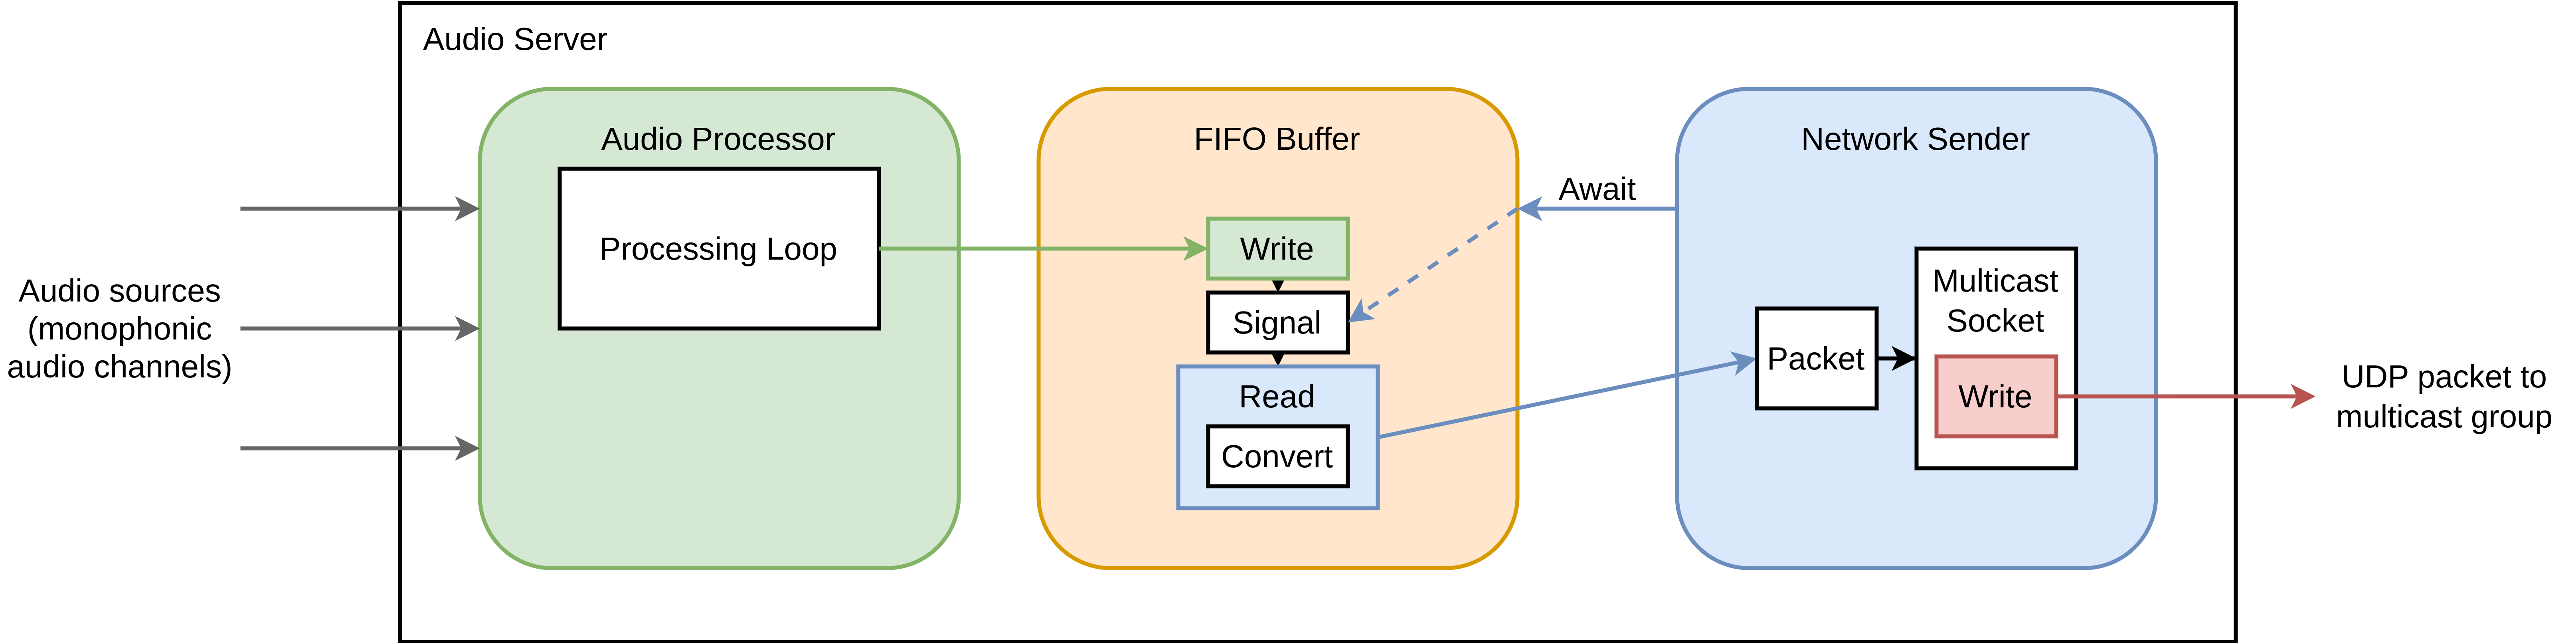
\includegraphics[width=\textwidth]{figures/audio-server}
    \caption{Overview of operation of the networked audio server.
    The network sender awaits notification of readiness to read samples from a
    first-in-first-out buffer of audio samples.
    The audio processor receives audio channels from a multichannel source
        (e.g. a DAW); at each iteration of its processing loop, it writes samples
        to the FIFO; upon write-completion, the FIFO sends a signal to the network
        sender that a block of samples is ready.
        Samples are converted to the appropriate format, and bundled into a UDP
        packet which is then written to the network.}
    \label{fig:audio-server}
\end{figure}

The networked audio server was written in C++ using utility classes provided by
the JUCE framework for the development of audio applications.\footnote{
    JUCE 7.0.5 \url{https://github.com/juce-framework/JUCE}
}
The server is encapsulated as a class called \texttt{NetAudioServer},
which can be incorporated into any JUCE-based audio application;
initial development was conducted on a basic console application, and later work
targeted a DAW plugin comprising a consolidated audio server and wave field
synthesis controller.

The \texttt{NetAudioServer} instance expects to receive blocks of
multichannel audio from an audio application's main processing loop.
It sets up network \textit{sender} and \textit{receiver} execution threads, and
assigns a network socket to each; a socket is essentially a numerical identifier
for an \textit{``endpoint for [network] communication''}
~\citep{noauthor_socket2_nodate} to which a type, such as \texttt{SOCK\_STREAM}
for TCP on \texttt{SOCK\_DGRAM} for UDP, can be assigned.
To avoid potentially blocking the audio application's main processing thread
with networking operations, upon receiving an audio block the server writes it
to an intermediate buffer \textemdash{} a first-in-first-out (FIFO) structure
\textemdash{} and signals to the sender thread that a block is ready for
transmission.
The sender thread, which as been awaiting such a signal, then requests samples
from the FIFO; these are stared as contiguous channels of 32-bit floating point
samples and converted, when requested, to the bit resolution specified in a
packet header created when \texttt{NetAudioServer} is initialised.
Upon receiving the requested samples, the sender thread writes these to its
socket, which has been configured to connect to a UDP multicast group.

\lstref{listing:audio-packet} shows an example network capture of an outgoing
audio packet:

\codeinputlisting[float=h]
{text}
{listings/audio-packet.txt}
{Network capture: ethernet frame containing a UDP audio packet}
{audio-packet}

Bytes \texttt{0x0000} to \texttt{0x0029} comprise the ethernet, IPv4, and UDP
headers, including the destination address: at position \texttt{0x001e}, the
bytes \texttt{0xe004e004}, or \texttt{224.4.224.4}, a valid (and unassigned)
UDP multicast address from the second ad-hoc address block as specified in the
IANA multicast address assignment guidelines~\citep{meyer_iana_2010}.
The six subsequent bytes are the header inserted into the packet by
\texttt{NetAudioServer}.
In \lstref{listing:audio-packet} these are:
\begin{itemize}
    \item \texttt{0xdf1c}: a sequence number (little-endian) of \numDec{7391};
    \item \texttt{0x04}: buffer size \numDec{4} corresponding with
    \texttt{BUF16};
    \item \texttt{0x02}: sampling rate \numDec{2} corresponding with
    \texttt{SR44};
    \item \texttt{0x02}: bit resolution \numDec{2} corresponding with
    \texttt{BIT16};
    \item \texttt{0x02}: \numDec{2} audio channels.
\end{itemize}

Audio data begins at byte \texttt{0x0030}.
Since the header indicates that there are two channels of 16-bit audio, and a
buffer size of 16 (samples, or rather frames of two channels worth of samples),
it is clear that the data for channel 1 encompasses the 32 bytes from
\texttt{0x0030} to \texttt{0x004f}, and channel 2 the remaining bytes.

Here, channel 1 is a test signal, a unit amplitude-increment unipolar sawtooth
wave, i.e.\ a signal whose amplitude starts at zero, and increments by 1 at each
sample until it reaches the maximum value that a signed 16-bit integer may take
\textemdash{} \numDec{32767} \textemdash{} at which point it wraps around to
zero and repeats.
This test signal serves two important purposes.
First, its impulse-like behaviour once every \num{32768} samples (roughly
\qty{.74}{\s} at a sampling rate of \qty{44.1}{\kHz}) is useful for taking basic
synchronicity measurements, e.g.\ involving connecting two clients' audio
outputs to an oscilloscope.
Second, this numerically-predictable signal served as a means to inspect the
integrity of the audio server algorithm, and to identify the appropriate
endianness for transmission.
Inspecting the first sixteen samples of the first audio channel (grouped
by sample for legibility, see \lstref{listing:chan-1-samples}), it is evident
that the amplitude values increment on a per-sample basis, and, since it is the
first byte that increases with each sample, that samples are transmitted little
endian.

\codeinputlisting[float=h]
{text}
{listings/audio-packet-excerpt.txt}
{Extracted samples from the transmitted unipolar sawtooth wave}
{chan-1-samples}

The receiver thread polls its socket for traffic reaching the multicast group
from clients, and uses the presence of an incoming packet stream as proof that
a client is connected.

\subsection{The Networked Audio Client}\label{subsec:networked-audio-client}

\begin{figure}[ht]
    \centering
    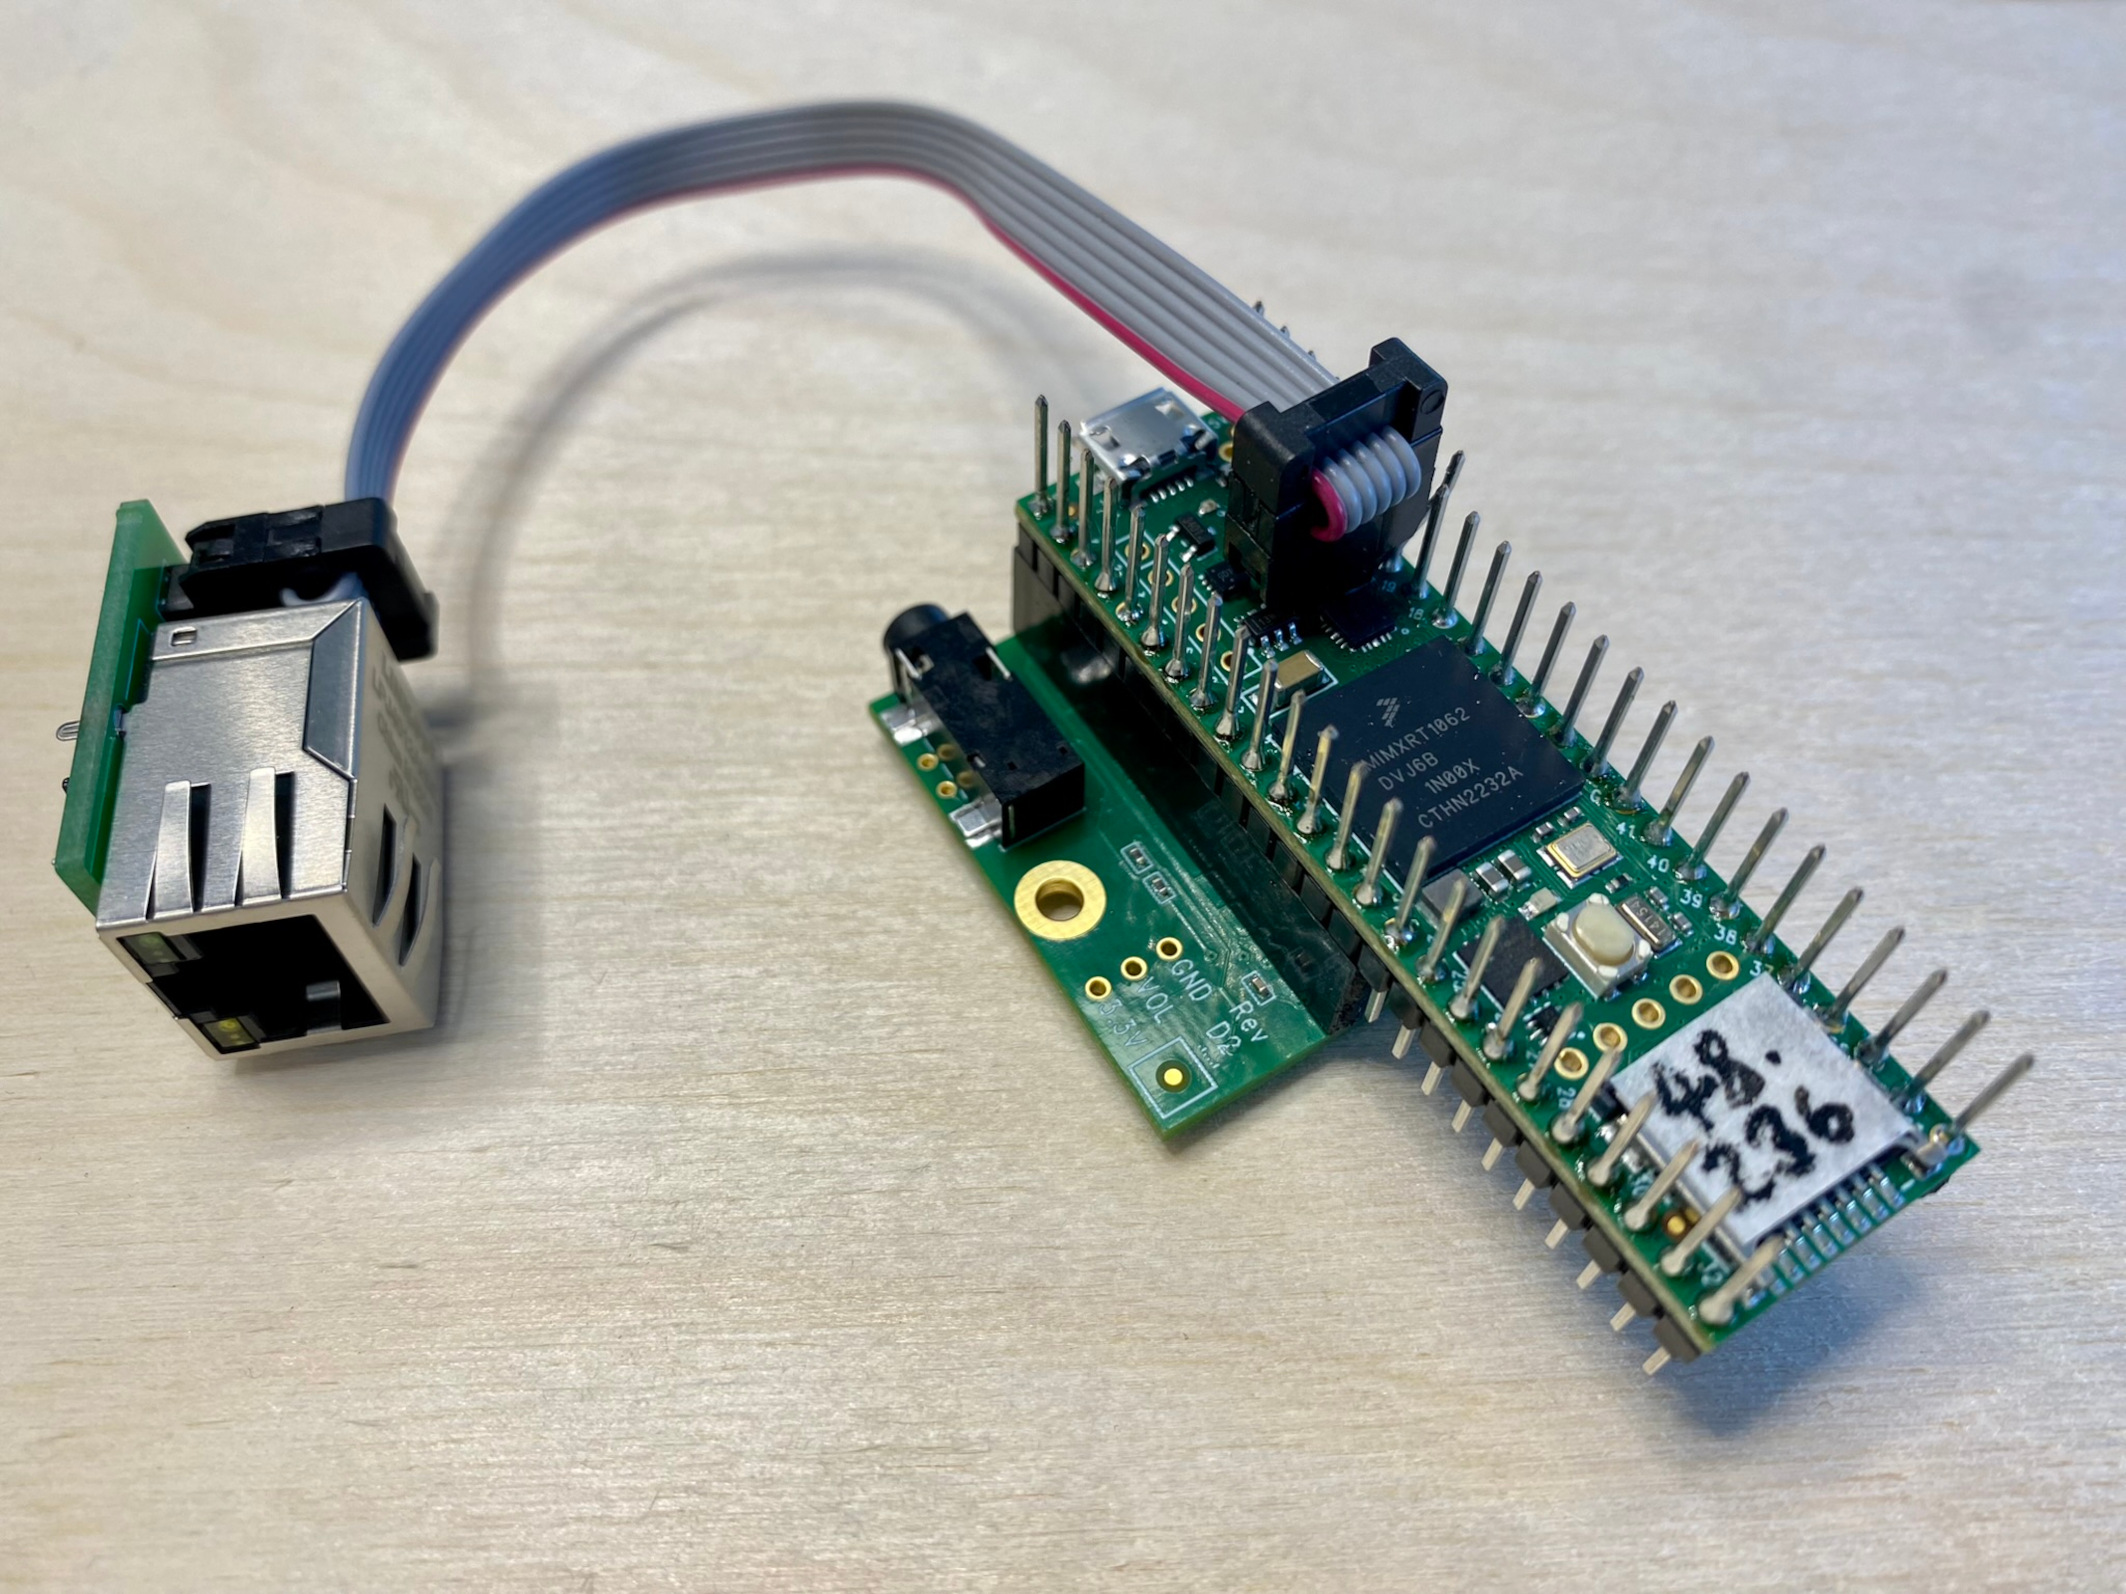
\includegraphics[width=.75\textwidth]{figures/module}
    \caption{A hardware module consisting of Teensy 4.1 microcontroller
        (labelled with the last two bytes of its serial number-derived IP address),
        connected via headers to an audio shield and via ribbon cable to an
        ethernet shield.}
    \label{fig:teensy}
\end{figure}
\noindent
Unlike the networked audio server, which runs on a general purpose computer and
has access to threads of execution, which it can use to conduct related but
separate tasks that rely on some central resource (the FIFO buffer alluded to
above), the client implementation is designed to operate on a microcontroller
platform that has no operating system, and no native notion of threads\footnote{
    There is in fact a non-core library, \textit{TeensyThreads}, that provides
    thread-like functionality. It was experimented with during development,
    but found to be incompatible with the interrupt-driven nature of the
    Teensy audio and networking libraries.
}.

The task of the network audio clients is threefold in nature:
\begin{enumerate}
    \item to retrieve packets of audio data from the UDP multicast group;
    \item to send a stream of audio data back to the multicast group, primarily
    to announce their connectivity;
    \item to maintain, as far as possible, synchronous operation with the
    server, and (by extension) each other.
\end{enumerate}

To address the first two requirements, the client sets up a socket, which it
uses to both read from and write to the UDP multicast group.

The client was created as a C++ class named \texttt{NetJUCEClient}, an
implementation of the Teensy audio library class \texttt{AudioStream}.
\texttt{AudioStream} descendents must implement a method named
\texttt{update()}; this method is called at each audio hardware interrupt, and
is where an audio library class should perform operations on the current
audio buffer.
Due to the regular timing of calls to \texttt{AudioStream::update}, and the
correspondence between an audio buffer and a network audio packet, it was
tempting to use that method, and thus the underlying audio interrupt, as an
opportunity to handle networking operations too.
This proved unreliable, however; conflicts between the audio and network
interrupts caused the Teensy to crash sporadically.

Instructions to read from and write to the network were moved to a method,
\texttt{NetJUCEClient::loop}, which is called from the top level loop of
the Teensy program.
Although not called at regular intervals \textemdash{} Teensy's \texttt{loop()}
function is itself executed from the body of a non-terminating \texttt{while}
loop \textemdash{} tests indicated that the time between iterations lay on the
order of tens of microseconds, far lower than the audio interrupt interval.

Separating audio and networking operations to \texttt{update()} and
\texttt{loop()} methods respectively, the two sets of operations were linked
by way of an intermediate buffer, similar to the FIFO used on the server.
Thus the client attempts to receive packets from, and send a packet to, the
multicast group on each call to \texttt{loop()}, with incoming packets written
to the intermediate buffer:

\begin{codelisting}{
    \texttt{loop} method of the networked audio client implementation,
    minted style=xcode,
    minted language=cpp,
    label=ls:njc-loop,
    float=h
}
    void NetJUCEClient::loop() {
        receive();

        checkConnectivity();

        send();

        adjustClock();
    }
\end{codelisting}
\noindent
The client also performs a periodic check for the presence of the server (and
potentially other clients),
and, as described in \secref{subsec:client-sync}, makes adjustments to its
audio clock.

On the audio interrupt, the client reads from the intermediate buffer to
produce samples for audio output.
It also takes samples reaching its audio inputs (e.g.\ arriving from other
Teensy audio library classes), and adds those to a packet to be sent to the
multicast group at the earliest possible subsequent call to
\texttt{NetJUCEClient::loop}:
\begin{codelisting}{
    \texttt{update} method of the networked audio client implementation,
    minted style=xcode,
    minted language=cpp,
    label=ls:njc-update,
    float=h!
}
    void NetJUCEClient::update(void) {
        doAudioOutput();

        handleAudioInput();
    }
\end{codelisting}

\subsection{Synchronicity with the Server}\label{subsec:client-sync}

Due to the influence of clock drift and transmission jitter, and since the
clients constitute a distributed system, with no direct knowledge of each other
and no authoritative source of time, their third task posed, without doubt,
the greatest challenge.

A two-pronged strategy was developed for addressing server-client and
inter-client timing discrepancies:

\textbf{Jitter Compensation:}
Similar to the approach taken in prior
work~\citep{rushton_microcontroller-based_2023}, clients monitored the difference
between the write and read positions to their intermediate audio buffer,
using a delay-locked loop to keep this difference within an interval of one
audio buffer.
This was achieved by way of setting thresholds for the read-write difference,
and adjusting the read-position increment if it fell beyond those thresholds;
increasing the increment if the difference exceeded the high threshold;
decreasing it should the difference fall short of the low threshold.
This in turn entailed employing a fractional read-position, and interpolating
around the read-position to achieve an appropriate sample value; essentially
a form of adaptive resampling.
For this purpose a cubic Lagrange interpolator was used; sample values for the
interpolator were converted from their 16-bit signed integer representation
to floating point numbers, interpolation conducted, and the resulting value
rounded to the nearest integer for output.

\textbf{Clock Drift Compensation:}
In the absence of an authoritative source of time, clients were set up to infer
the difference in rate between their own internal clock and that of the server
by comparing the rate of packet reception from the network to their internal
audio interrupt rate.
This was achieved by taking the ratio, over thirty-second intervals, of
packets written from the network to the intermediate buffer to blocks read
from the intermediate buffer for audio output.
This ratio was then used to calculate appropriate divisors to apply to the
\qty{24}{\MHz} master clock generated by a crystal oscillator on the Teensy,
adjusting the audio clock's phase locked loop (PLL) to produce an adjusted audio
sampling rate.
The aim of this approach was to minimise reliance on the adaptive resampler
described above, and ultimately encourage all clients to run at the same audio
rate as the server.

\subsubsection{An Unexpected Source of Jitter}

Jitter does not arise solely during the journey from machine to machine across
a network.
It was found that, using the general purpose computer's default audio host
(ALSA), the timing of iterations of JUCE's audio processing loop, and thus
signals to \texttt{NetAudioServer}'s sender thread, was very uneven, i.e.\
subject to a high degree of jitter.
Though the average rate of execution was commensurate with the selected sample
rate and audio buffer size, individual audio buffer intervals differed, in
microsecond terms, by up to an order of magnitude. This inconsistent audio
timing was sufficient to cause transmission jitter that overwhelmed
the client-side strategy for jitter compensation.
The result was consistent audible distortion due to rapid fluctuations in the
client's audio buffer read-position increment.

Switching from ALSA to JACK as the audio host resolved this issue, but since
JACK \textit{uses} ALSA as its underlying audio host, this phenomenon was
difficult to account for.
A detailed description lies beyond the scope of this report, but
essentially JACK uses \textit{direct memory access} to map the underlying audio
device into memory,\footnote{
    Credit goes to Stéphane Letz, a prominent contributor to the JACK project,
    for providing this bit of context.
} and seemingly does so in a more effective manner than the driver
for the sound card on the development machine.
It is not known at the time of writing whether using ALSA with an external audio
interface (a potential barrier to entry) would have improved the situation.

This incident serves to illustrate that, beyond the concerns associated
with effective software design, a system such as the one described here, for
which the timing of operations is critical, is susceptible to the whims of
a variety of supporting hardware and software systems \textemdash{} things
that in a more conventional audio system can, to a greater degree, be taken for
granted.
The topic of whether to attempt to compensate for this sort thing in software
or impose strict requirements on a future end-user in terms the audio host they
should use (something that would almost certainly vary with the user's
operating system), remains one for future research.

\begin{figure}[ht]
    \centering
    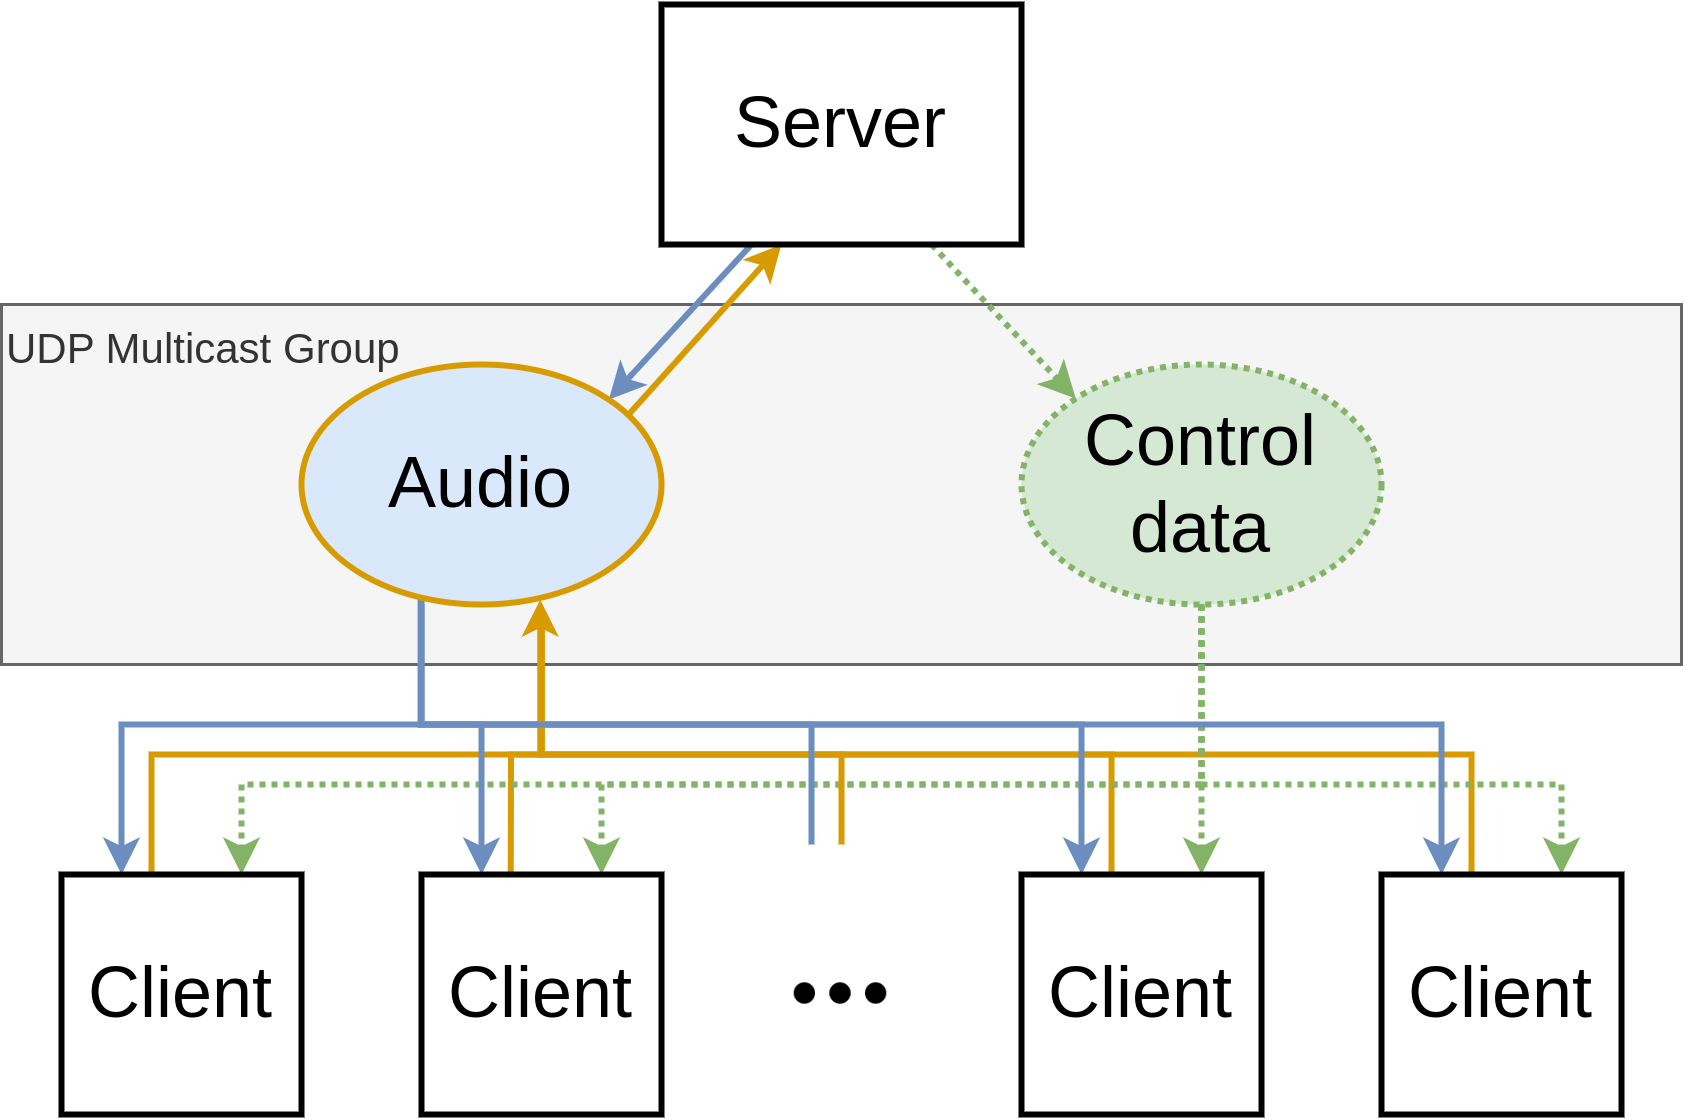
\includegraphics[width=.75\textwidth]{figures/multicast}
    \caption{Architecture of the networked audio system.
    The server sends audio and control data to a UDP multicast group on
    distinct port numbers; clients listen for this data, and send an audio
    stream back to the multicast group with which the server can register
    their presence on the network.}
    \label{fig:multicast}
\end{figure}

\begin{figure}[ht]
    \centering
    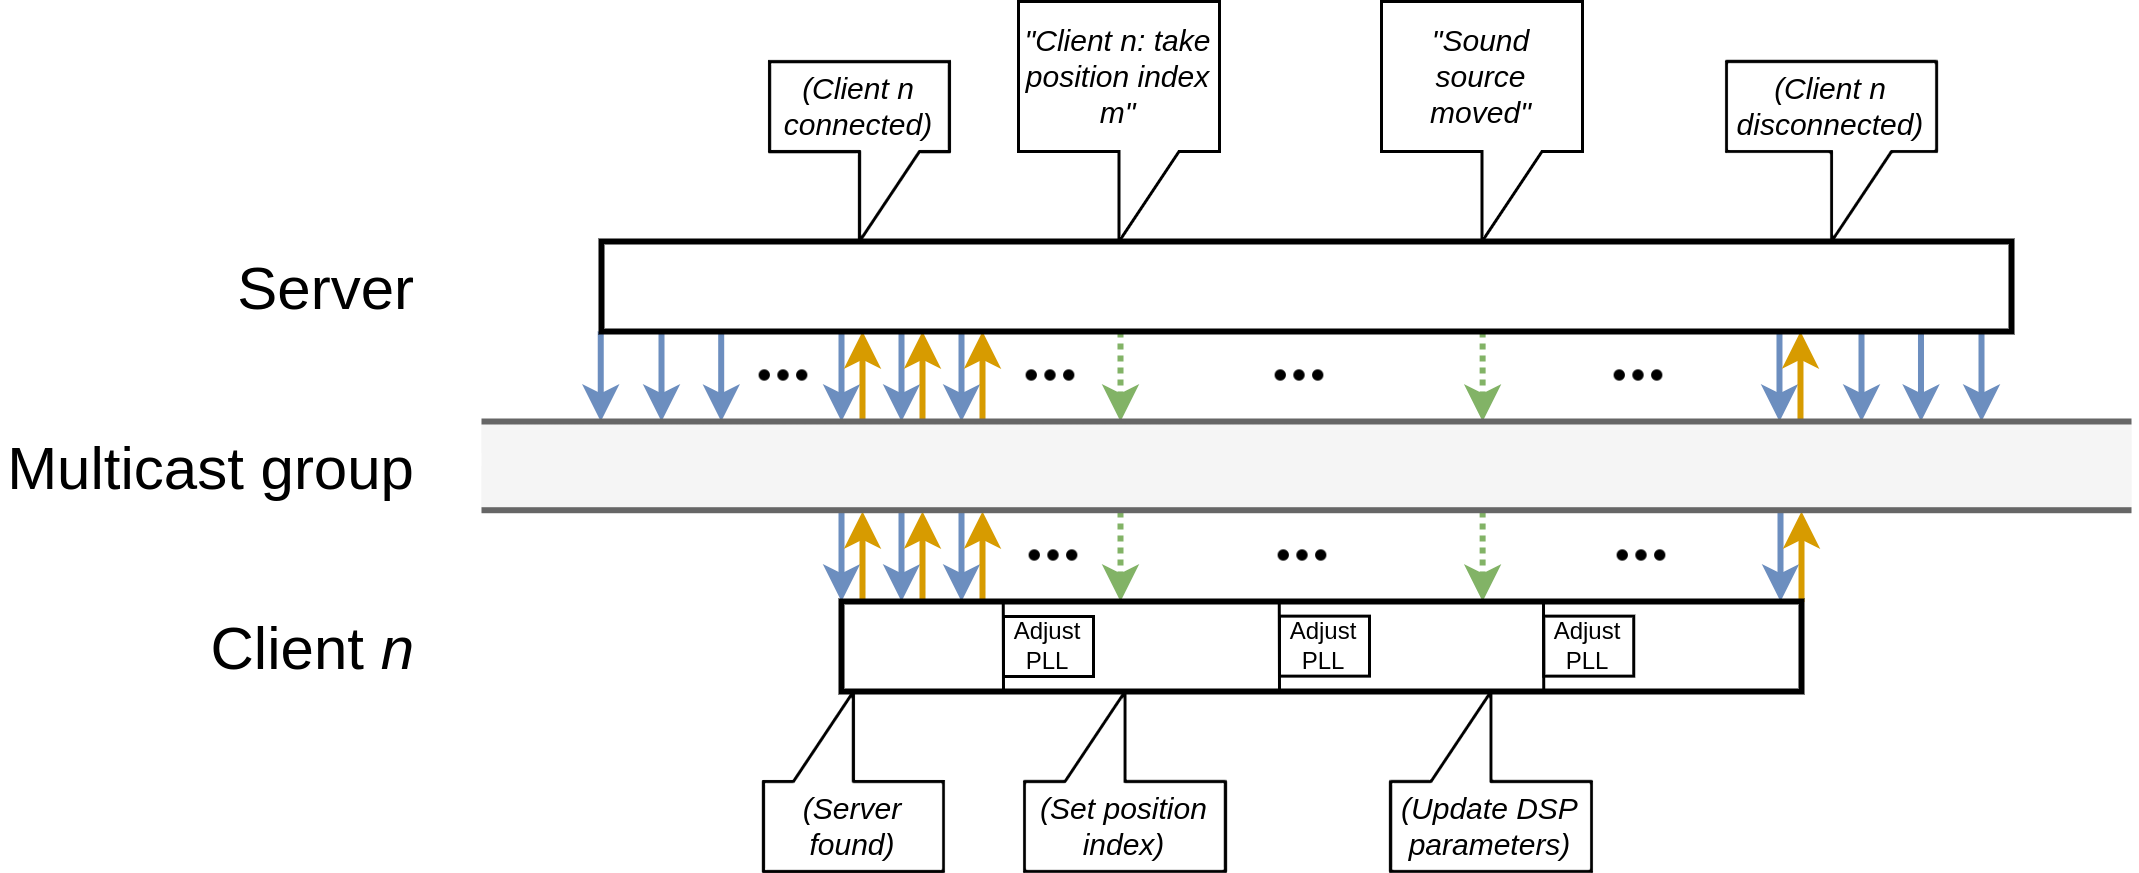
\includegraphics[width=\textwidth]{figures/timeline}
    \caption{Example timeline of client-server interaction. Blue arrows
    indicate audio data being sent from the server to the multicast group;
    orange arrows indicate audio data being sent from the client back to the
    multicast group;
    green arrows represent control data.}
    \label{fig:timeline}
\end{figure}

\subsubsection{A Note on the Client-Server Dichotomy}\label{subsubsec:client-server}

In principle, there is no meaningful impediment to the so-called
clients acting as servers in their own right; a change of port number is all
that would be required for each client to receive traffic from (and send
traffic to) not just the server, but also from (and to) all other clients.
Consequently, in code for both the server and clients, networked audio entities
in the system are referred to as \textit{peers} (see, e.g.
\figref{fig:plugin-interface}).
In practice, and for the particular application
\textemdash{} distributed spatial audio \textemdash{}
considered here, receiving UDP packets from sources other than the designated
server is not only unnecessary, but also manifestly inefficient.
With Chafe et al.'s \textit{Internet Acoustics} work in mind, it is likely that
there are some very interesting uses for a \textit{promiscuous} network
of audio peers, but, for now, such applications lie beyond the scope of this
work.

% \missingfigure{Diagram of signal format conversion, transmission, reception,
%     and re-conversion, i.e. UDP packets, sample buffers.}

\subsection{The Audio Spatialisation Algorithm}\label{subsec:wfs-algorithm}

With some minor modifications, e.g.\ the possibility to specify speaker spacing
parametrically, the WFS algorithm
from~\citep{rushton_microcontroller-based_2023} was reused.
This algorithm was written in Faust, a domain-specific programming language
for audio synthesis and signal processing\footnote{
    \url{https://faust.grame.fr/}
}, and compiled to
a C++ class compatible with the Teensy audio library via Faust's
\texttt{faust2teensy} utility~\citep{michon_real_2019}.

\todo[inline]{Talk about the teensies were programmed; mention tytools.}

Implementing Huygens' principle in a digital audio system entails applying
delays to an audio signal representing a virtual sound source based on the
intended position of that sound source with respect to the secondary point
sources.
To limit the computational burden placed on the hardware modules, specifically
with regard to memory, the length of the delay lines was reduced by discarding
the longitudinal component of $r_k$, leaving only the relative inter-speaker
delay.
Additionally, a simplified WFS prefilter was employed, using the distance
from each virtual sound source to each secondary point source to an inverse
square law mapping for frequency-independent amplitude loss to the medium of
propagation, and the cutoff of a two-pole lowpass filter.
Adopting a modified version of equation~\eqref{eq:driving-function}, the
driving function becomes:
\begin{equation}
    \label{eq:simple-driving-function}
    d_k(\bfx,t) = f(t, r_k) \ast \delta\left(t - \frac{r_k-y_k}{c}\right).
\end{equation}
In implementation, the prefilter was tuned by ear using Faust's
\texttt{fi.lowpass} function\footnote{
    \url{https://faustlibraries.grame.fr/libs/filters/\#filowpass}
};
a thorough treatment of the simulation of distance effects in WFS stands as a
topic for future work.

\subsubsection{Modularity and Maximum Delay}

The reduction in the maximum delay length represented by the subtraction of
the longitudinal distance component in
equation~\eqref{eq:simple-driving-function} is essential for the viability of
the system.
As capable a platform as Teensy 4.1 is, as described in
\secref{subsec:hardware-platforms}, it is limited in terms of memory.
This in turn places limits on the lengths of delay lines that it can compute,
a matter exacerbated if there are many such delays to consider, such as in the
case of a WFS implementation with numerous virtual sound sources.
Each hardware module must compute two delay lines for each virtual source, one
for each of its output channels, the maximum length of which (depending on
the position of a given module in the speaker array) corresponds, after removal
of the longitudinal component, of the width of the speaker array.
It was observed that, for eight virtual sources and eight hardware modules,
the maximum speaker spacing permissible lay around \qty{.4}{\m},
corresponding with a speaker array of maximum width 15 $\times$ 0.4 =
\qty{6}{\m}, equating to a maximum delay of $\sim$\qty{17}{\ms} or
approximately 795 samples at a sampling rate of \qty{44.1}{\kHz}.
The matter has not been rigorously tested, but nonetheless the presumption is
that this places significant limits on the modularity of the system.
\todo[inline]{What about soldering on extra PSRAM?}
It is hoped that future versions of the Teensy platform, or developments in
other microcontroller platforms, overcome this manner of limitation.

\subsubsection{Controlling the WFS Algorithm}

Parameter values are delivered to the Faust algorithm in the form of OSC
messages.
OSC control data, describing virtual sound source positions, speaker spacing,
and informing clients of their position in the speaker array, is bundled into
UDP packets and delivered by the server to the multicast group for all clients
to consume.

\codeinputlisting[float=h]
{text}
{listings/control-data-packet.txt}
{Network capture: ethernet frame containing a UDP control data packet}
{control-data-packet}

\lstref{listing:control-data-packet} demonstrates an example control data
packet, an OSC bundle containing one message.
This message has address \texttt{/source/0/x}, indicating that it refers to the
$x$-coordinate of the zeroth sound source, providing a value in the form of a
32-bit floating point number, \texttt{0x3d1b5fa2}, approximately
\numDec{0.038}.\todo[inline]{Check control data endianness}

\subsection{System Overview}\label{subsec:system-overview}

Being composed of multiple hardware and software components, it is worthwhile
to summarise the nature of these components and the interactions between them.

\subsubsection{Hardware Setup}

The network audio server runs on a general purpose computer.
During the development and testing of this project, that computer was an ASUS
G513R Notebook PC, with an AMD Ryzen 7 6800H processor with a clock
speed of \qty{3.2}{\GHz}.
For the majority of development, the computer's internal sound card was used;
for testing and evaluation, it was connected to a Steinberg UR44C USB audio
interface in the hope that this would provide better reliability in terms of
audio interrupt timing.

The computer was connected via CAT6 ethernet cable to an eight-port ethernet
switch (D-Link DGS-108GL).
For evaluation, and to support a total of eight network audio clients, this
switch was daisy-chained to an additional switch (D-Link DES-1008D).
Teensy 4.1 hardware modules, assembled as per \figref{fig:teensy}, were
connected via CAT6 ethernet cables to available ports on the ethernet switches.
Hardware modules were powered by a combination of a seven-port USB hub, plus,
for the eighth module, a USB mains socket.
The two audio outputs of each hardware module were connected to M-Audio BX5
speakers.

\subsubsection{Software System}\label{subsubsec:software-system}

\begin{figure}[ht]
    \centering
    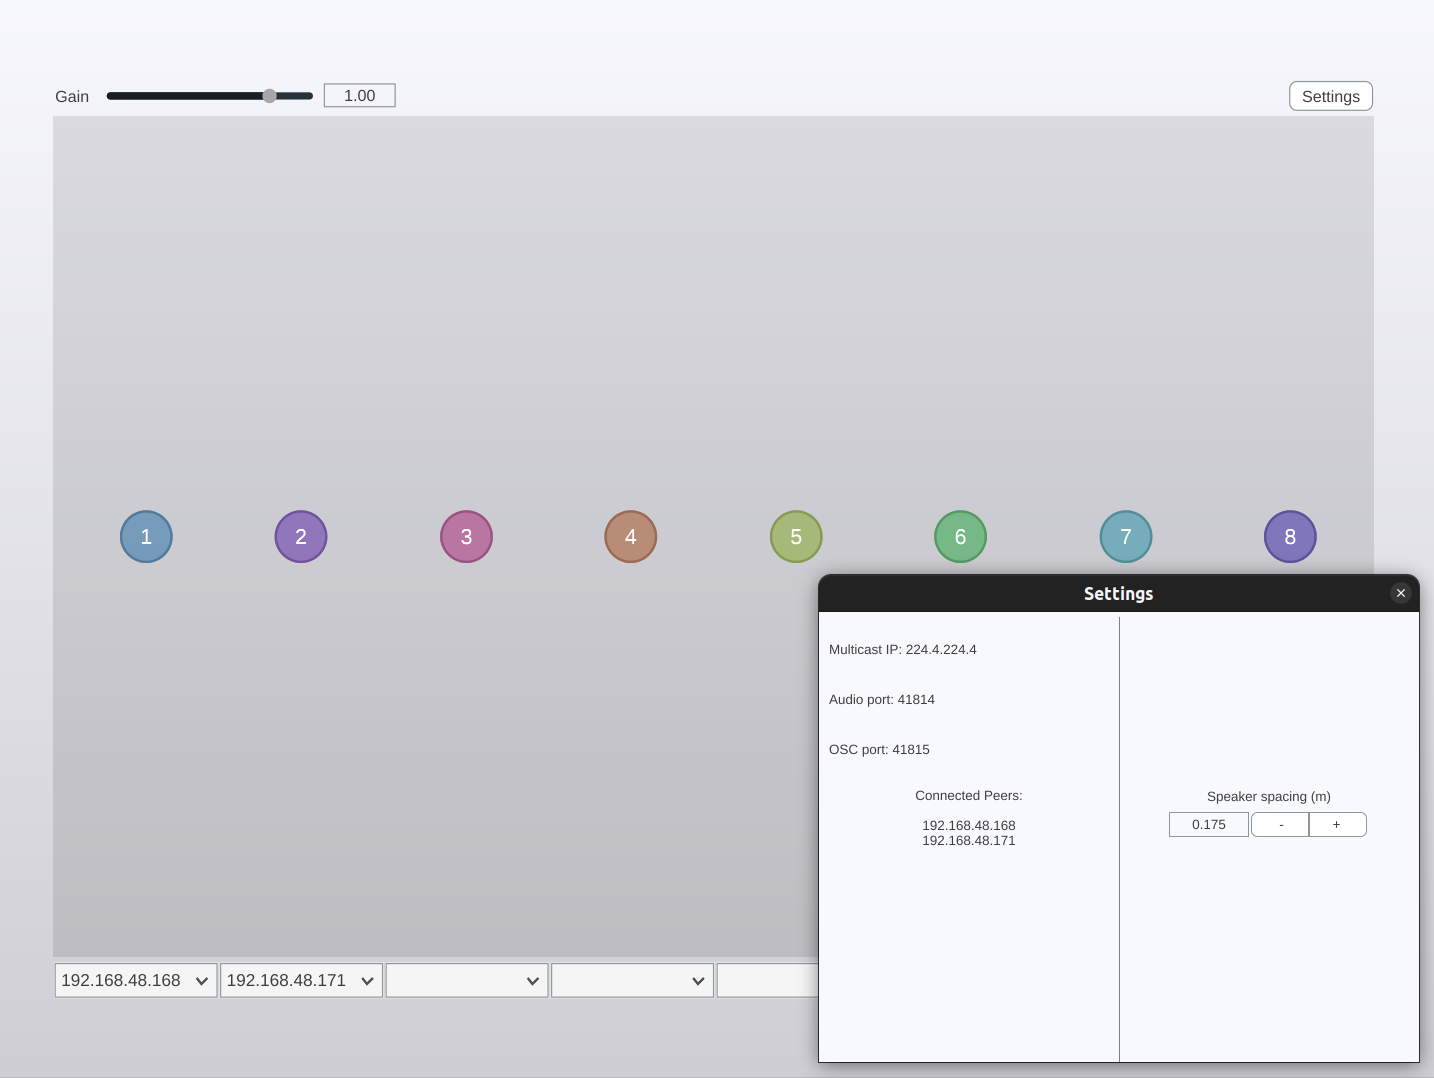
\includegraphics[width=\textwidth]{figures/plugin}
    \caption{
        User interface for the WFS controller DAW plugin, with modal
        settings window visible.
        The interface consists of an X/Y control surface, with eight nodes
        representing the locations of sound sources in a virtual sound field.
        Dropdown menus at the bottom of the interface correspond with hardware
        module positions in the loudspeaker array.
        The settings window facilitates specifying the speaker spacing, and
        shows a list of connected network peers.
    }
    \label{fig:plugin-interface}
\end{figure}

Server-side, the software system consists of a VST plugin running in Reaper
digital audio workstation software\footnote{\url{https://reaper.fm/}}.
The plugin comprises the networked audio server, receiving monophonic audio
sources in the form of audio or instrument tracks in the DAW, plus a control
data server, commanded either by parameter automation via the DAW, or manually
via a graphical user interface (see \figref{fig:plugin-interface}).
The audio and control data servers send streams of UDP packets to a UDP
multicast group.

Client-side software connects to the multicast group and reads UDP packets
containing audio and control data from the server.
These streams are delivered to the Faust-based WFS algorithm, with audio
streams processed according to the control parameters of virtual sound source
positions and speaker spacing.
The WFS algorithm produces driving signals for each of the two output channels
of the hardware module on which it is running.
Additionally, the client-side networked audio client returns a stream of audio
data to the multicast group, to be consumed by the server.

Code for the server and client software components can be found at
\url{https://github.com/hatchjaw/netjuce} and
\url{https://github.com/hatchjaw/netjuce-teensy} respectively.\todo[inline]{
    Document code repos.
}

% \begin{figure}[ht]
%     \centering
%     \includegraphics[width=\textwidth]{figures/system-overview.jpg}
%     \caption{System overview.}
%     \label{fig:system-overview}
% \end{figure}


    \section{Results}\label{sec:results}

\begin{figure}[ht]
    \centering
    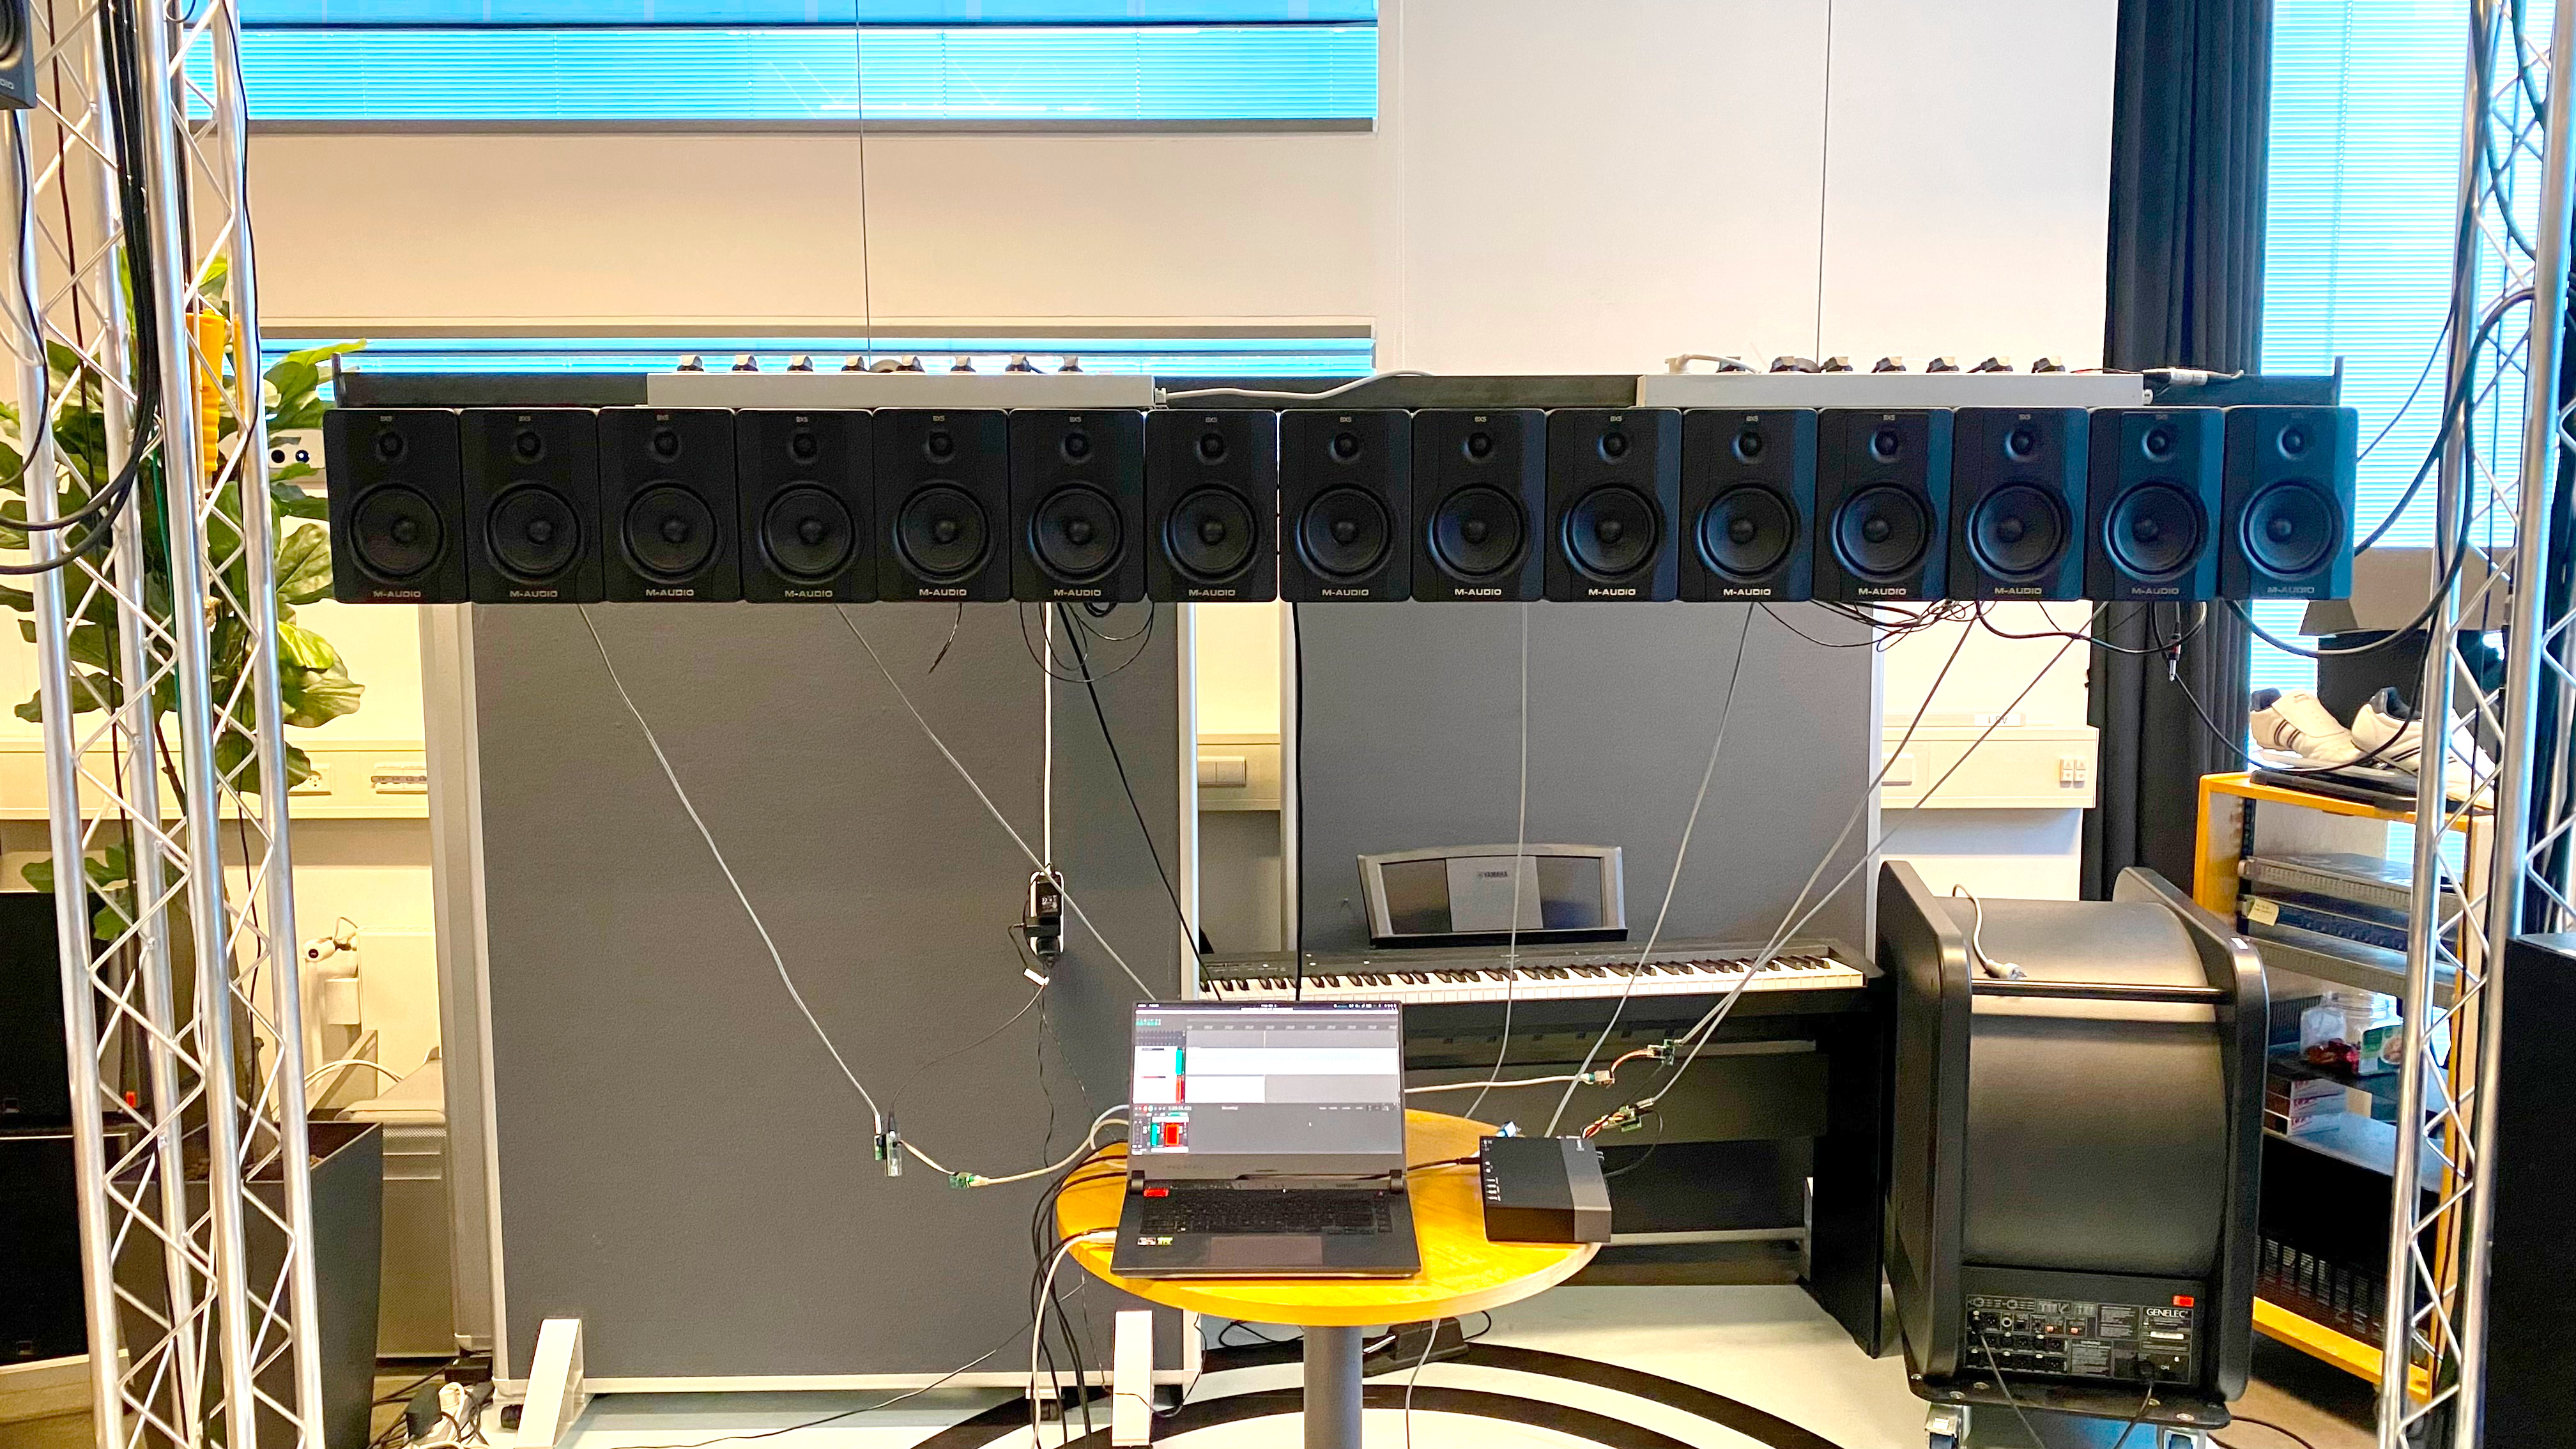
\includegraphics[width=\textwidth]{figures/eval-setup}
    \caption{
        System configuration for technical and perceptual evaluation.
        Eight hardware modules connected to fifteen loudspeakers \textemdash{}
        seven of the modules produced output for two loudspeakers each; the
        final module used only its first output channel.
    }
    \label{fig:eval-setup}
\end{figure}

Possessing technical underpinnings, but ultimately being designed to
serve immersive auditory ends, it was important to consider the performance of
the system described and developed in \secref{sec:method} in terms of
both its technical capabilities and the quality of the perceptual effects it
was able to support.
The success of the system as platform for audio spatialisation techniques is
contingent on it being composed of effective solutions to the challenges posed
by distributing audio processing across a local area network.
It is of limited worth, however, as a technical exercise in isolation;
the subjective assessment provided by listeners exposed to its output may help
identify the most critical aspects of the technical implementation and guide
future development.

\subsection{Technical Evaluation}\label{subsec:technical-evaluation}

\begin{figure}[ht]
    \centering
    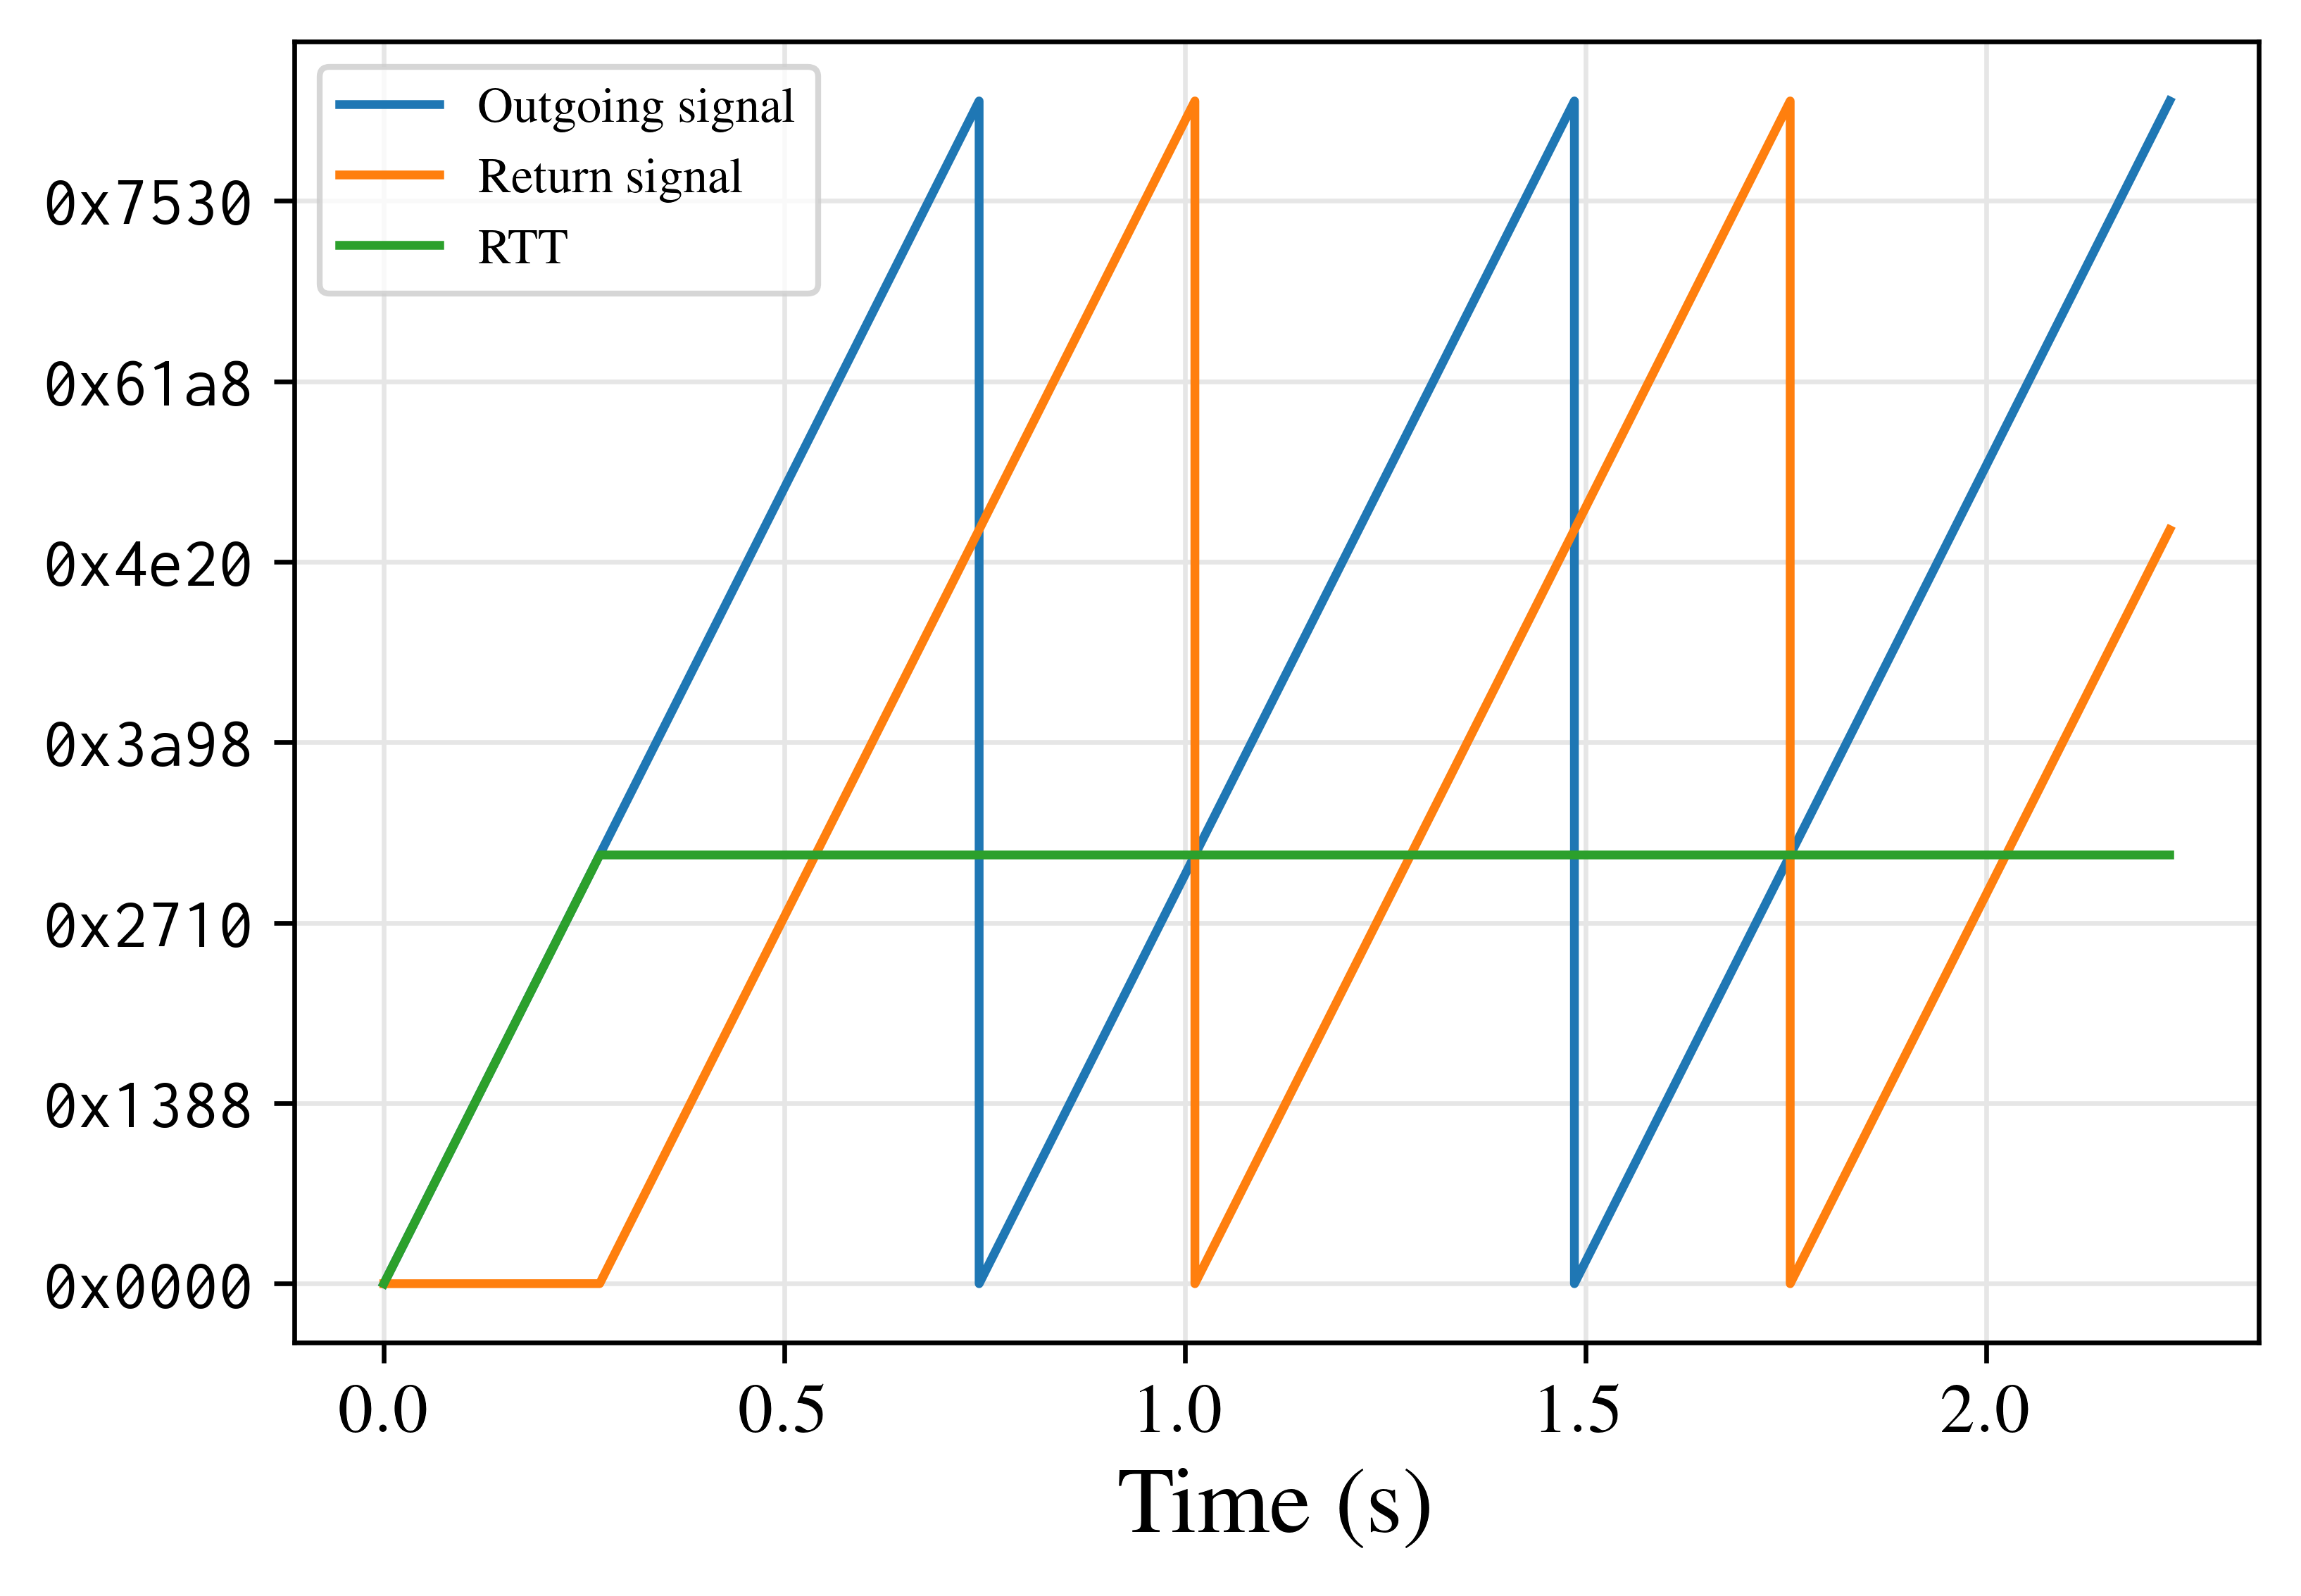
\includegraphics[width=.5\textwidth]{figures/test-signal}
    \caption{
        Illustration of the use of a test signal, a unipolar sawtooth wave,
        to measure round trip time.
        Subtracting the return signal from the outgoing signal gives the time
        (in samples) between transmission and reception.
    }
    \label{fig:test-signal}
\end{figure}
\noindent
Of most pressing technical concern is the matter of synchronicity between the
hardware modules.
To assess this, a similar approach was taken to that found
in~\citep{rushton_microcontroller-based_2023}
and~\citep{gabrielli_networked_2012}.

\subsubsection{Round Trip Time}
To measure transmission round trip time (RTT), the
server transmitted a unipolar sawtooth wave of unit amplitude increment to the
multicast group, and each client, upon receiving that signal simply returned it
immediately to that same group to be consumed by the server.
At the server side, the return signal, $x_{\text{ret}}$, was subtracted from the
outgoing signal, $x_{\text{out}}$, at the time of reception, with round trip
time found as:
\begin{equation}
    \label{eq:rtt}
    \text{RTT} = \begin{cases}
                     x_{\text{out}} + \max_{\text{int16}} - x_{\text{ret}}, &x_{\text{out}} < x_{\text{ret}}, \\
                     x_{\text{out}} - x_{\text{ret}}, &\text{otherwise},
    \end{cases}
\end{equation}
where $\max_{\text{int16}}$ is the maximum value representable by a
signed 16-bit integer, \texttt{0x7fff} (\numDec{32767}).

The resulting value is the number of samples elapsed between transmission and
reception (see \figref{fig:test-signal}).
Since there is one source of transmission, for multiple clients, comparing RTT
offers a means to assess inter-client synchronicity.
Server-to-client latency cannot be measured in this way, but that can be
inferred to be around half of, and, of course, certainly not greater than, the
RTT.\

\subsubsection{Clock Drift/Skew}
A unipolar sawtooth wave of unit amplitude
increment was generated on the clients, subtracted from the incoming sawtooth
wave from the server, and the difference (found similarly to
equation~\eqref{eq:rtt}) returned to the multicast group for consumption by the
server.
Under ideal conditions, the incoming signal and the one being generated on a
given client, while not necessarily (and almost certainly not) synchronised,
should be out of phase by some constant value;
if this value changes then some relative drift has occurred between server and
client.
While not of direct relevance to synchronicity, the client-side clock-adjustment
strategy was designed to minimise the reliance on the adaptive resampling
approach that it complements;
low drift would be indicative of the effectiveness of that strategy.

\begin{figure}[ht]
    \centering
    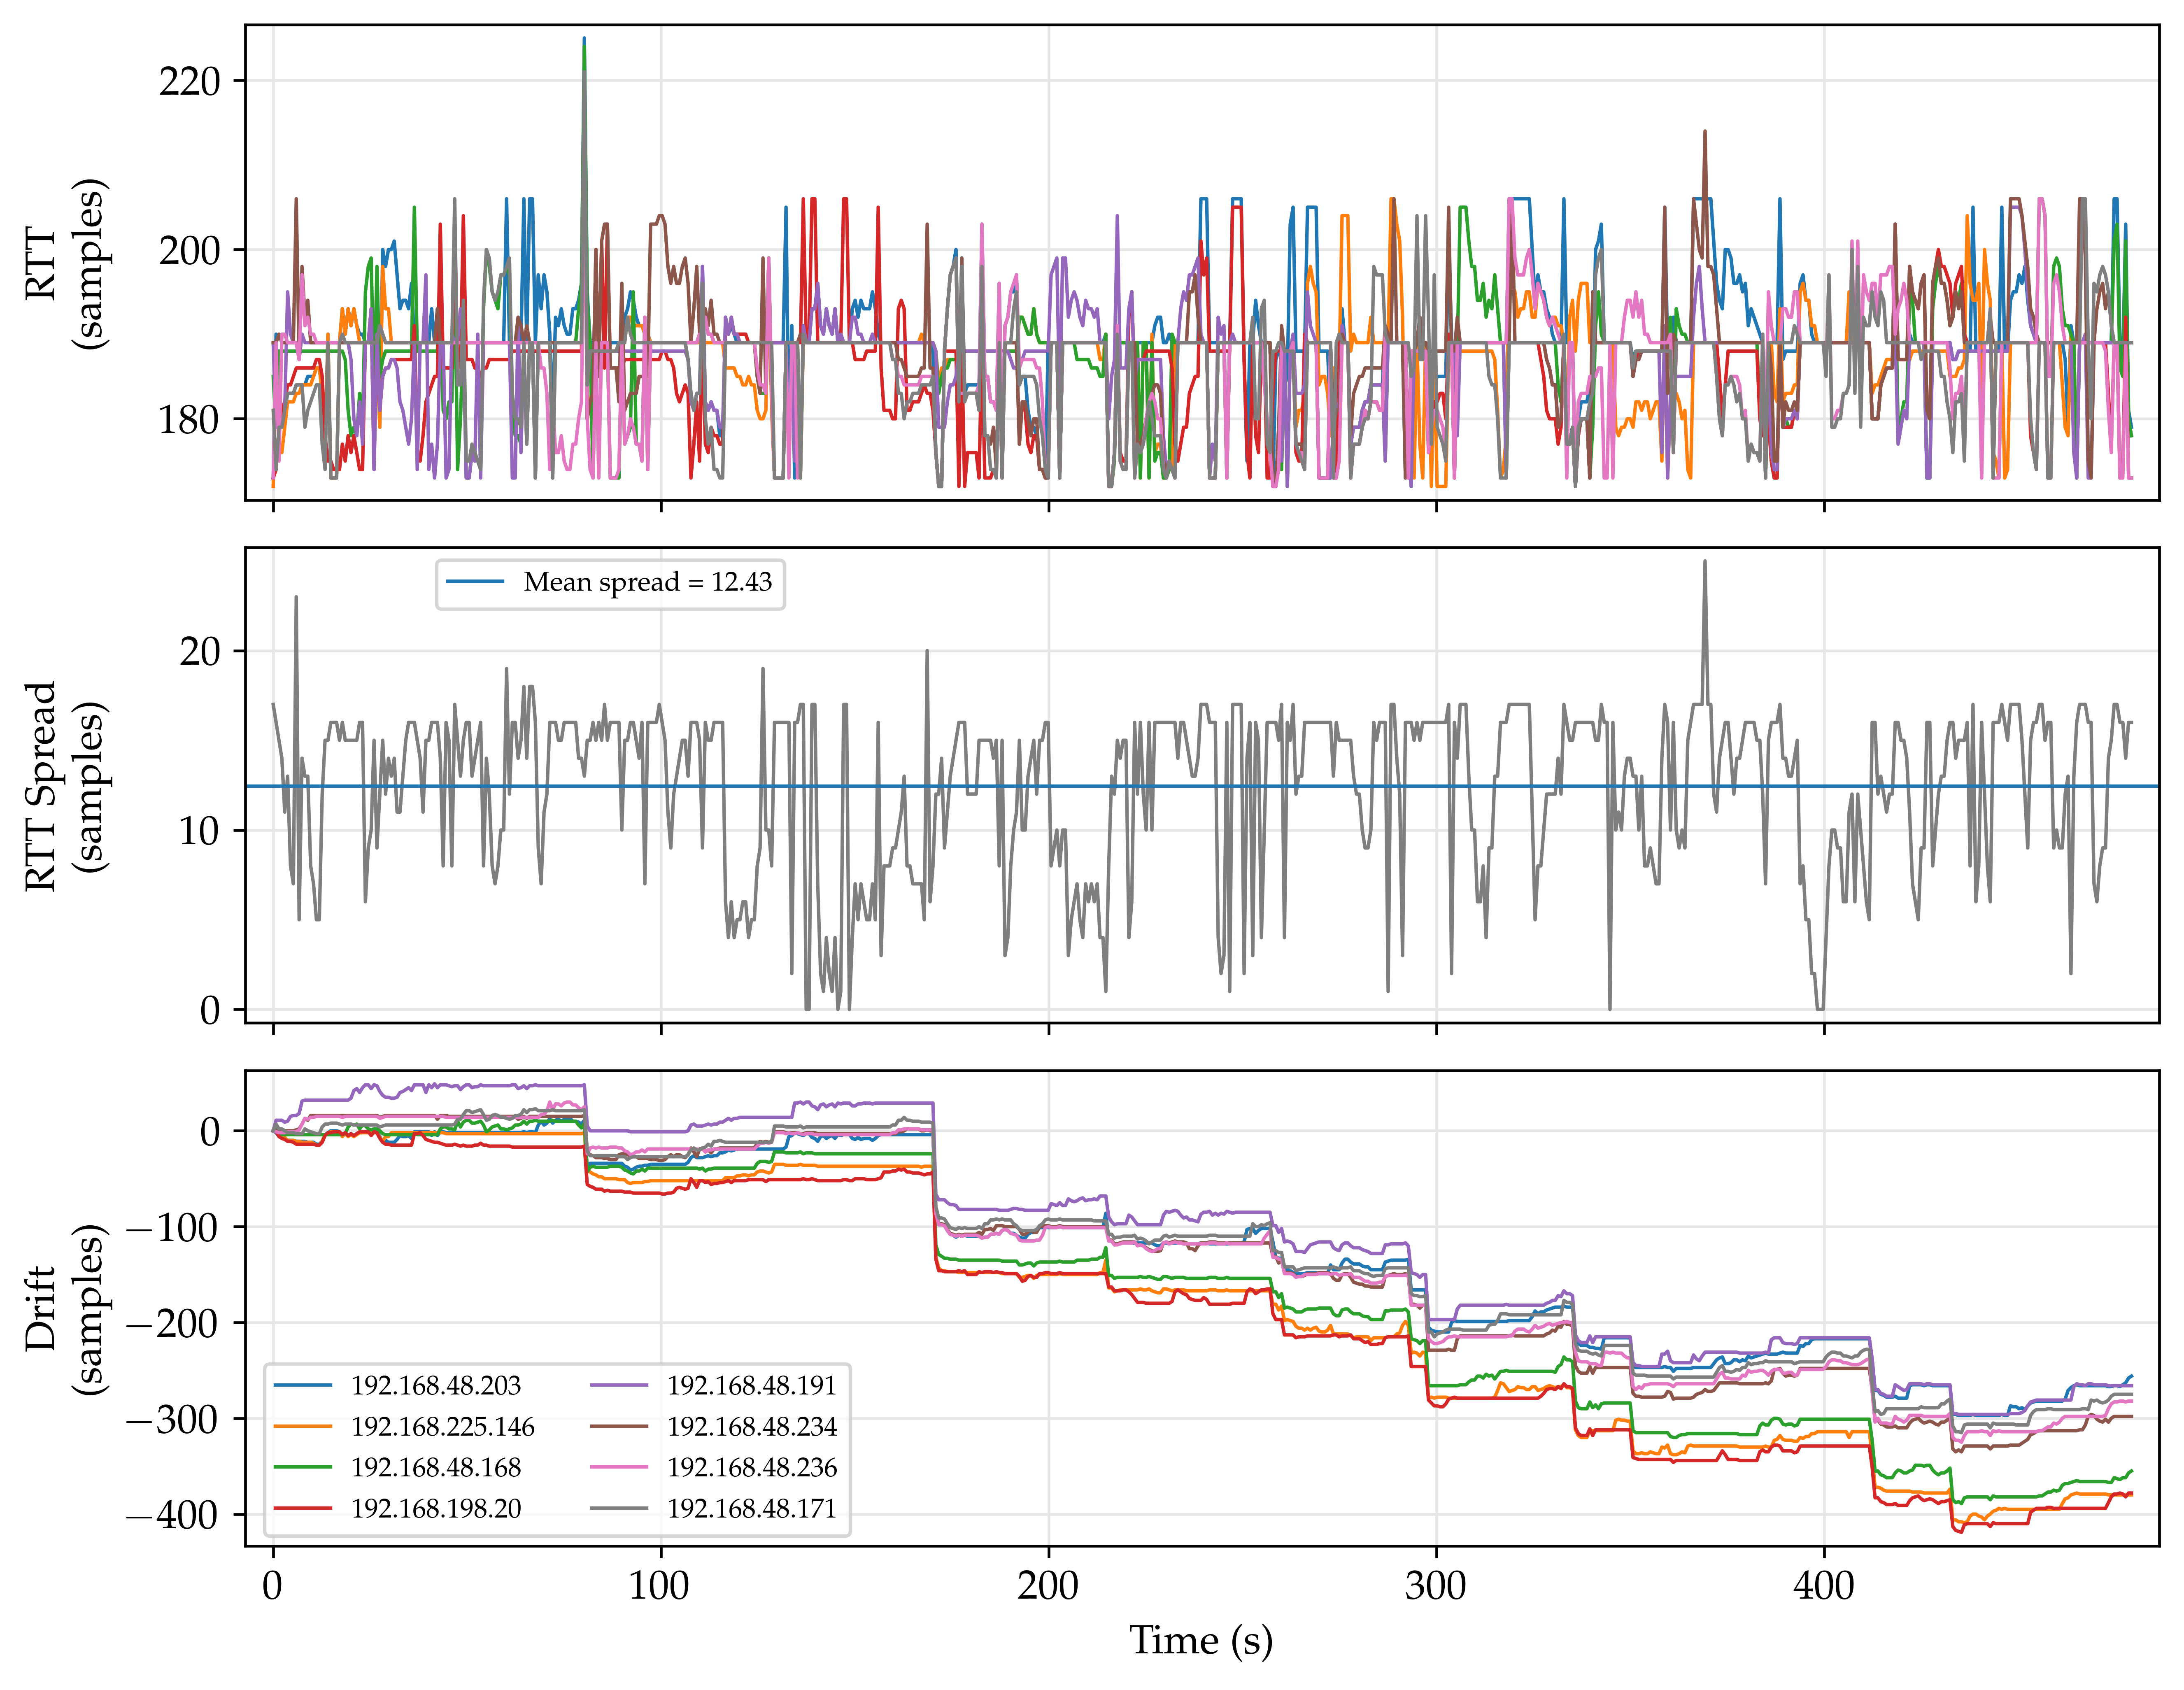
\includegraphics[width=\textwidth]{figures/rtt_drift_16}
    \caption{
        Round-trip time, RTT spread, and clock drift measurements for eight
        networked audio clients, for a networked audio session of eight minutes'
        duration.
        Audio buffer size, 16 samples.
    }
    \label{fig:rtt-drift-16}
\end{figure}

Initial RTT and relative drift measurements for eight clients are shown in
\figref{fig:rtt-drift-16}.
Mean RTT spread, describing the average temporal interval over which clients
were distributed over the course of the test, is promising, the 12.43 sample
interval corresponding with approximately \qty{282}{\us}.
RTT, and thus maximum latency, is clustered around a respectable 190 samples
($\sim$\qty{4.3}{\ms}).

That visual clustering, coupled with the apparent tendency for RTT spread to
lie at around 16 samples (i.e.\ precisely one buffer), suggest, however, a
certain over-aggressiveness in the resampling strategy, perhaps resulting in a
polarisation of clients to the temporal extremes of the interval between their
audio interrupts.
What \figref{fig:rtt-drift-16} does not show, and, given the short timescales
involved, is not easily represented in such a diagram, is the rate of relative
inter-client movement, i.e.\ the rate of change of asynchronicity.
Cursory, subjective assessment of the system's audible output revealed that,
given the rapid rate of relative movement between clients, in this state it
would not stand up to perceptual testing.

Transmitting a signal consisting of white Gaussian noise (WGN) to the clients
and delivering this to their audio outputs without further processing
\textemdash{} seeking, essentially, to sonify QoS \textemdash{} an
aggressive phasing, or time-varying comb-filter effect was clearly audible.
This effect is visualised in \figref{fig:spectrograms}(a); ideally (and
subject to the frequency of the response of the microphone used) an ambient
recording of a white noise source would correspond with a magnitude spectrogram
exhibiting equal intensity across the frequency range at all times; clearly,
though, there are regions of greater and lesser intensity, and these regions
shift and change rapidly over time.
In addition to the above, tests involving the reproduction of signals
containing steady-state harmonic content revealed obtrusive audible artefacts.

\begin{figure}[ht]
    \centering
    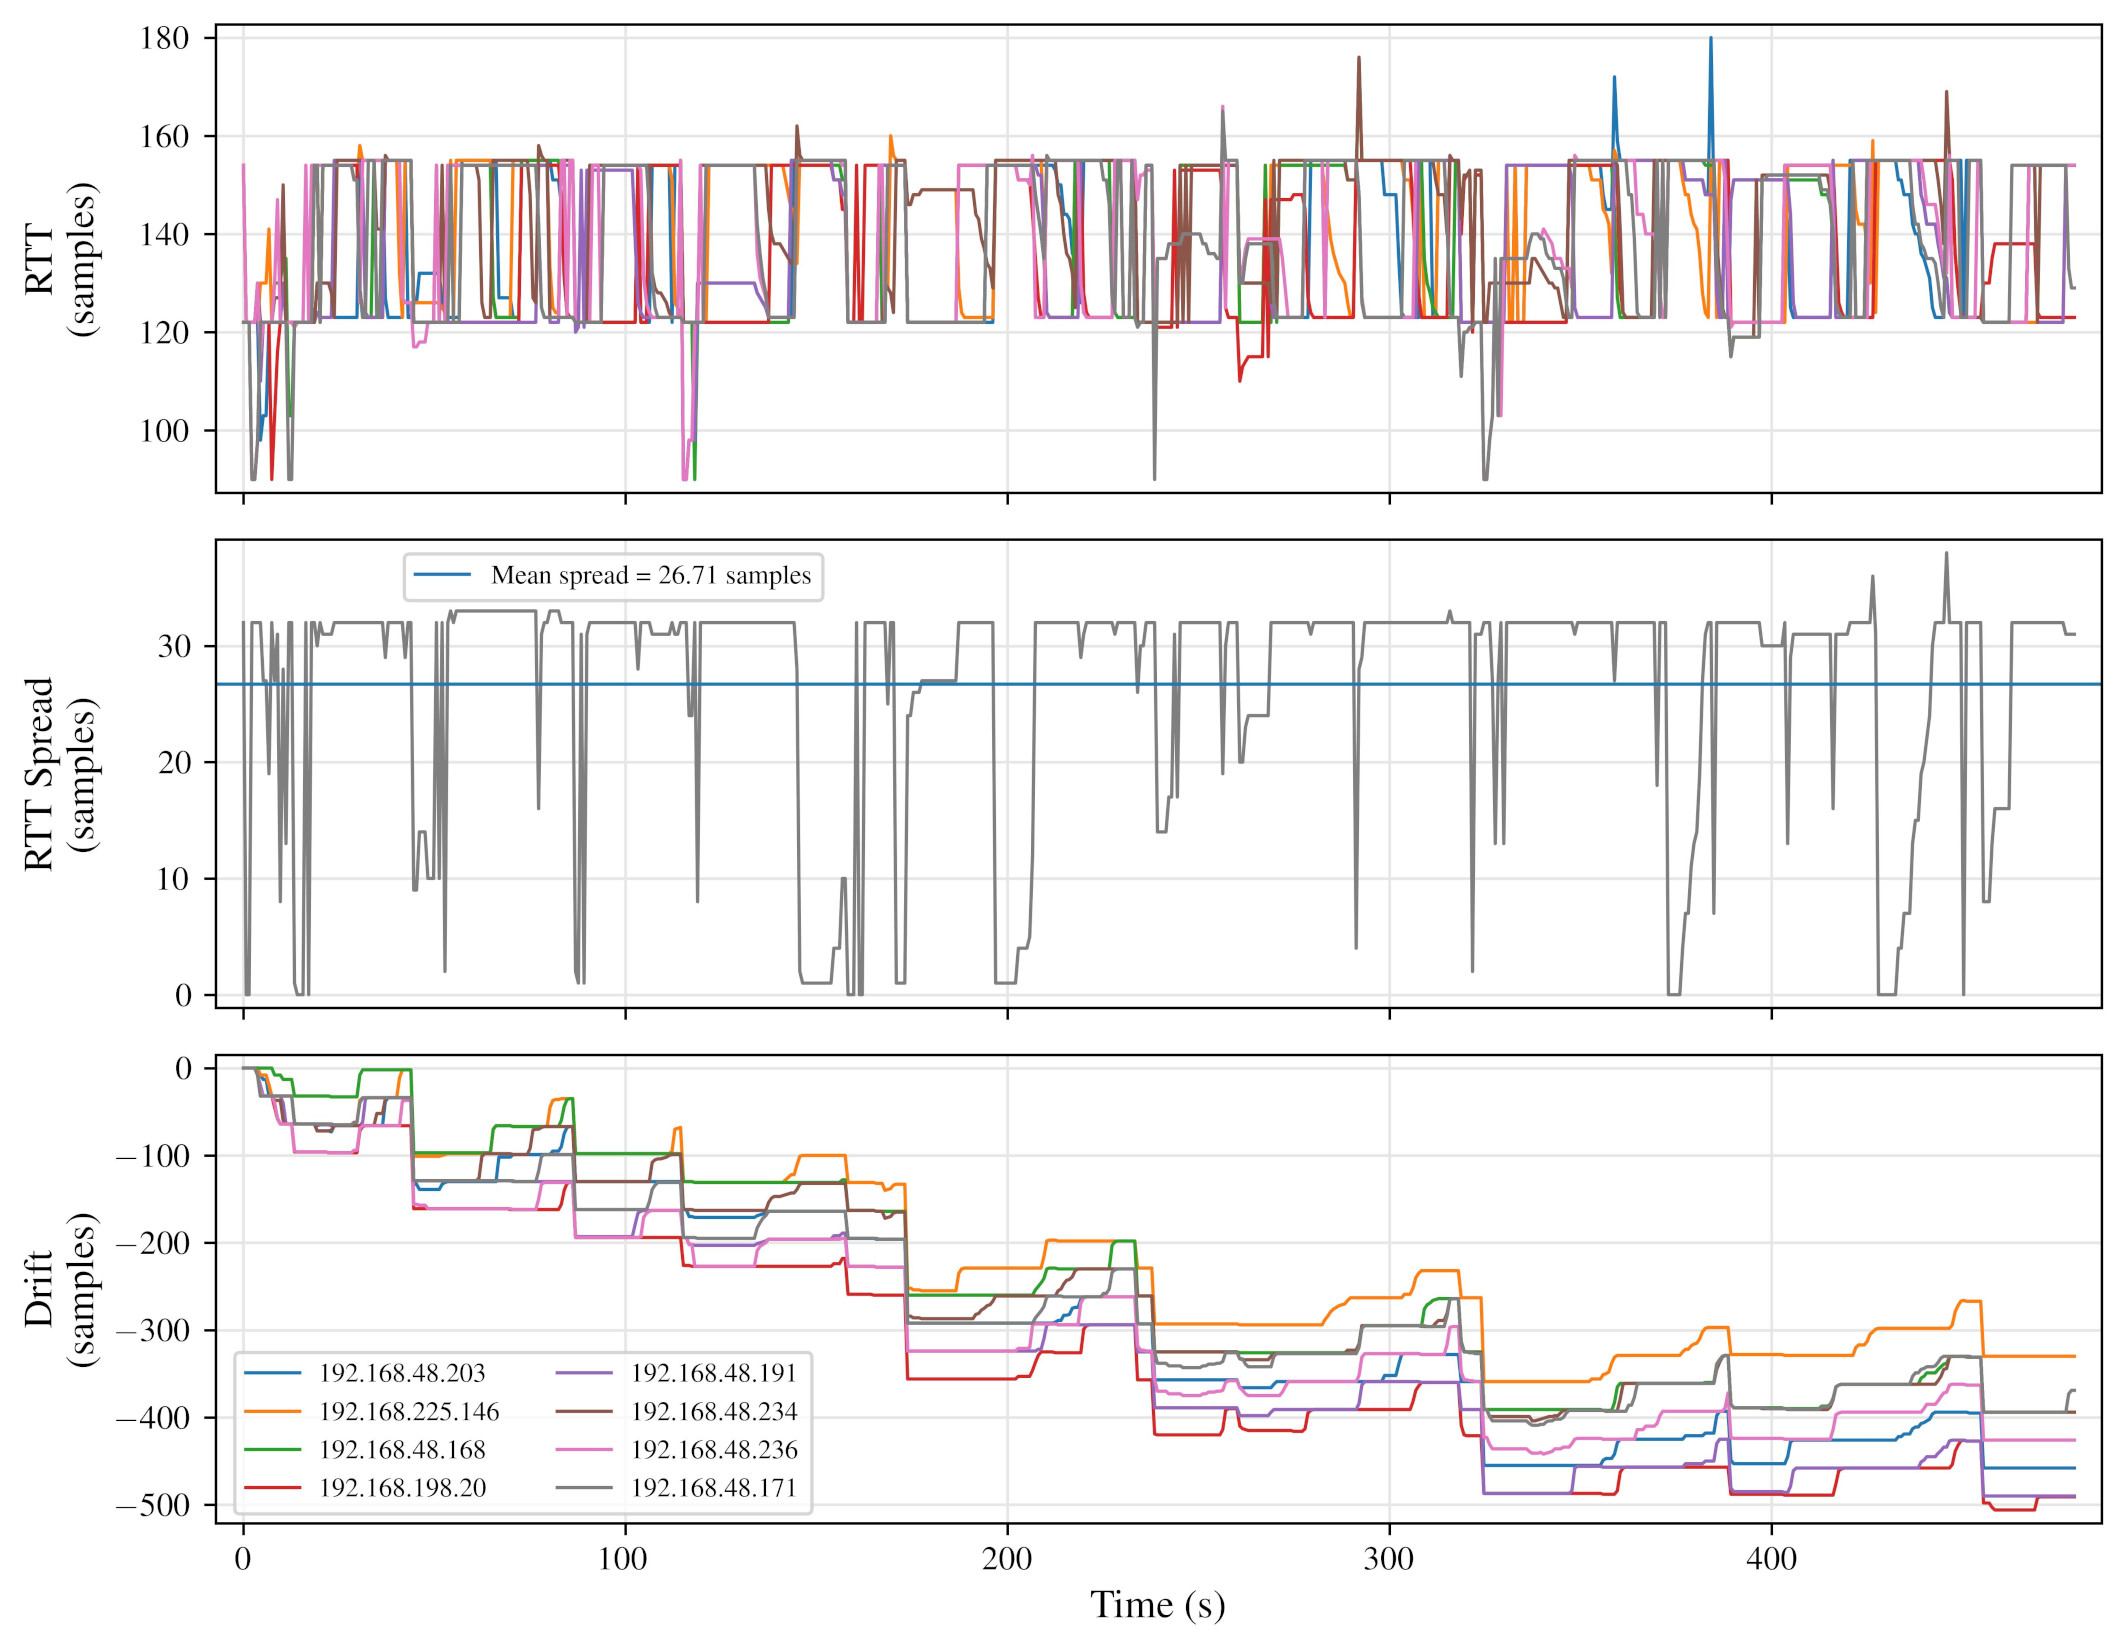
\includegraphics[width=\textwidth]{figures/rtt_drift_32}
    \caption{
        Round-trip time, RTT spread, and clock drift measurements
        for eight networked audio clients, for a networked audio session of
        eight minutes' duration.
        Audio buffer size, 32 samples.
    }
    \label{fig:rtt-drift-32}
\end{figure}

A buffer size of 16 samples had been selected in an attempt to minimise the
duration of the window of inter-client synchronicity, and to maximise the
number of channels that could be transmitted over the network, subject to
restrictions posed by the MTU (see
\secref{subsubsec:transmission-considerations}).
Recalling, however, that previous
work~\citep{rushton_microcontroller-based_2023}
had employed a 32-sample audio buffer, equivalent measurements were taken for
the larger buffer size, the results of which are depicted in
\figref{fig:rtt-drift-32} and \figref{fig:spectrograms}(B).

\begin{figure}[ht]
    \centering
    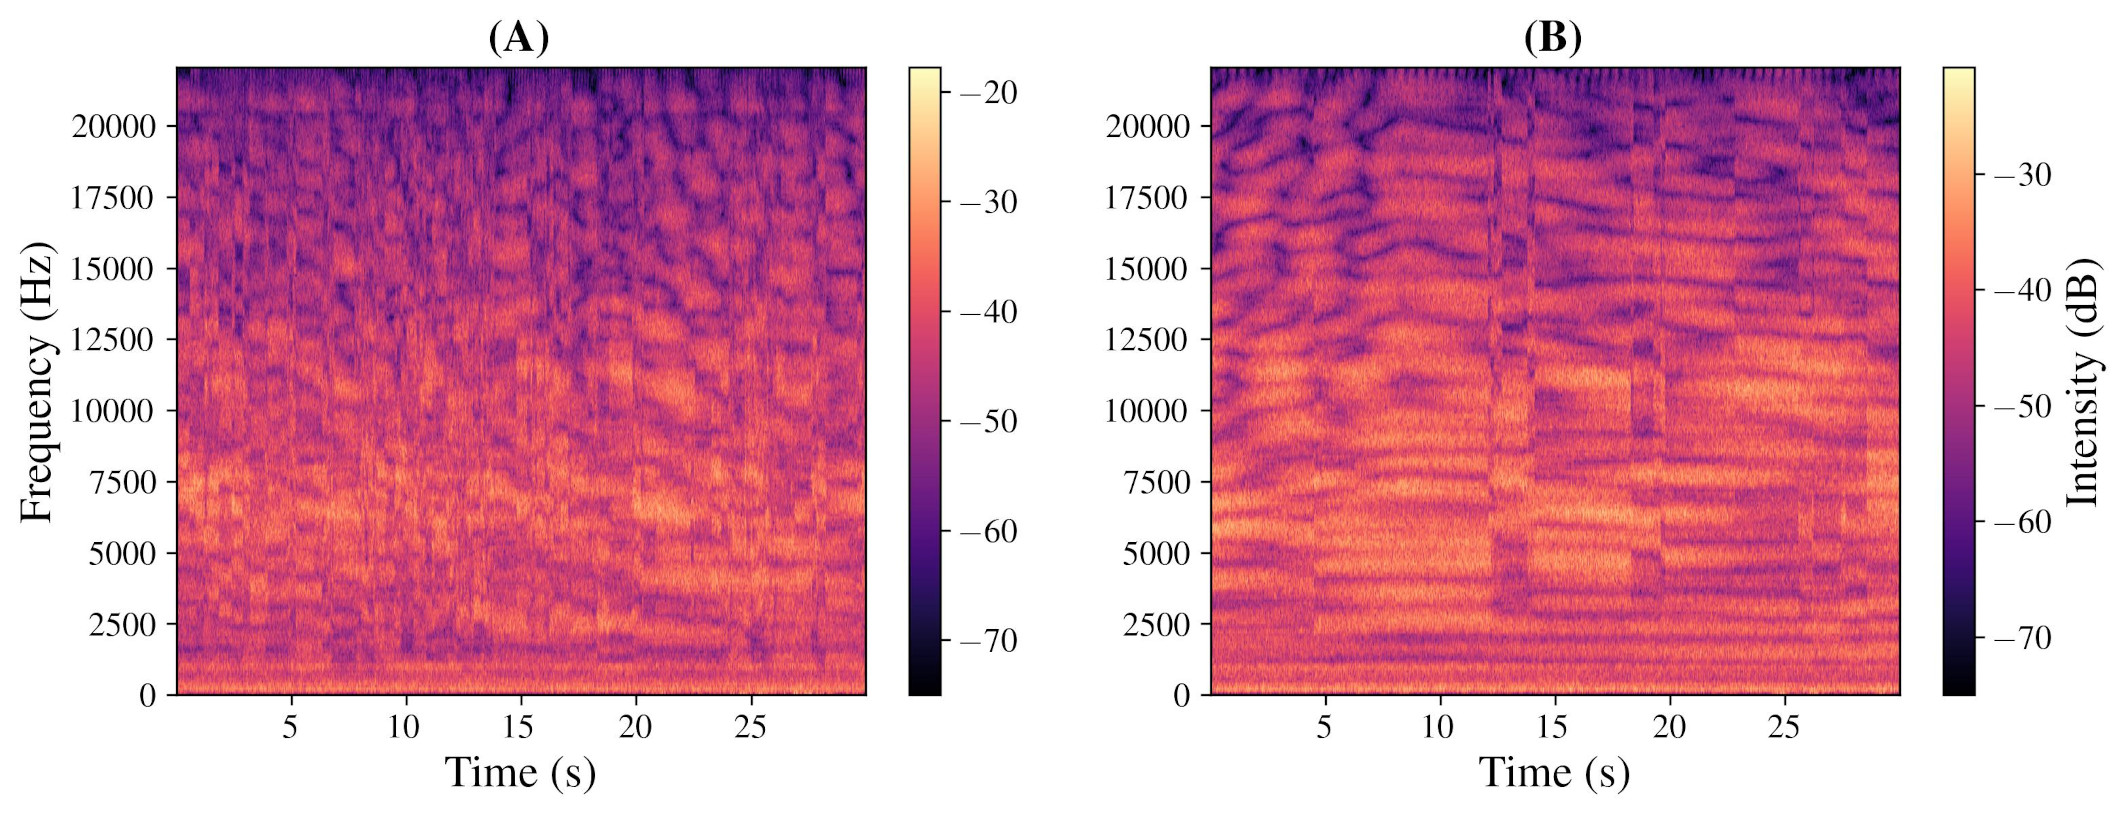
\includegraphics[width=\textwidth]{figures/wgn_specgram_16_32}
    \caption{
        Magnitude spectrograms of ambient, monophonic recordings of a
        reproduction of white Gaussian noise by a group of eight networked
        audio clients driving an array of fifteen loudspeakers spaced at
        intervals of \qty{.175}{\m}.
        Capacitor microphone placed $\sim$\qty{2}{\m} from the
        speaker array.
        Audio buffer (and thus network packet) size (A) 16 samples;
        (B) 32 samples.
    }
    \label{fig:spectrograms}
\end{figure}

Again, visually, there is an apparent clustering in the RTT recordings, with
clients spending large periods separated by around one buffer's worth of
samples ($\sim$\qty{726}{\us}), seemingly often grouped at either
extreme of the interval of one audio buffer.
The mean RTT spread, $\sim$\qty{626}{\us}, is comparable with results
from prior work, but, disappointingly, slightly less favourable.
Importantly, however, and as demonstrated in \figref{fig:spectrograms}(B), the
rate of relative inter-client temporal movement was much improved by the switch
to a 32-sample buffer.
Although exhibiting similar visual striations to the spectrogram for the test
at 16 samples, fluctuations occur less frequently, and seemingly more
gradually.
Indeed, subjectively-speaking, the disruption caused by the phasing effect
that afflicted the 16-sample buffer implementation was significantly reduced,
as was the presence of audible artefacts affecting harmonic signals.
Thus it was the version of the system employing a buffer size of 32 samples
that was exposed to perceptual evaluation.

Clock drift measurements in \figsref{fig:rtt-drift-16}{fig:rtt-drift-32} exhibit
comparable trends.
Increasing negative drift over time is indicative of the clients running faster
than the server.
Visually, there is evidence that client clocks adjust to approximate parity
with the server for periods of time, perhaps falling slightly slower (e.g.\
the drift plot in \figref{fig:rtt-drift-16}, between 100 and 160 seconds), but
periodically demonstrate large negative steps.
These leaps are far from desirable, and suggestive of there being significant
room for improvement in the devised strategy for PLL adjustment.


\subsection{Perceptual Evaluation}\label{subsec:perceptual-evaluation}

The WFS system was subjected to an informal perceptual evaluation, in which
participants were presented with a virtual sound source at various locations
and asked to indicate, on a diagram of the virtual sound field, the point
at which they estimated the sound had emanated from.
The informality of the experiment arose in part as a consequence of the
listening environment not being acoustically treated, and there being sources
of ambient sound in the laboratory in which the WFS system was installed.
Furthermore, the speaker array (\figref{fig:eval-setup}) consisting of fifteen
speakers, but each hardware module producing two audio output channels,
the second channel of the right-most module was not used;
for eight modules, however, the WFS plugin assumed a virtual sound field
spanning sixteen speakers, thus it was possible to position a virtual sound
source horizontally beyond the rightmost extent of the speaker array.
Ultimately the aim of the experiment was to draw some preliminary, guiding
conclusions as to the effectiveness of the distributed WFS system in
triggering listeners' localisation cues, its technical and installation
shortcomings notwithstanding.

In terms of the design of the auditory stimulus, it was felt that listeners
would be most comfortable localising a naturalistic sound.
Rather than use blasts white noise as in~\citep[ch.~6]{verheijen_sound_1998},
but wishing to minimise the potential effects of frequency-dependent
localisation interference due to spatial aliasing, a broadband stimulus
was selected in the form of a close-mic recording of a snare drum.
The recorded sample was repeated three times in succession at intervals of
\qty{.125}{\s}, and, again in the interests of adding a natural quality to the
sound, with slight variations in amplitude (the second iteration of the sample
was played marginally quieter than the first; the third slightly louder).

Participants were given a brief description of the system under evaluation,
and informed that they should expect to hear sounds that appeared to emanate
from `behind' the speaker array, from which they stood at a distance of
$\sim$\qty{2}{\m}.
Eight different virtual source positions were specified via automation of the
$x$ (lateral) and $y$ (longitudinal distance) components of the position of a
node in the WFS plugin interface.
The range of the $x$ component corresponded with the distance from the driver
of the leftmost speaker to the centre of the driver of the missing sixteenth
loudspeaker; drivers lay at intervals of \qty{.175}{\m}, giving a horizontal
axis spanning \qty{2.625}{\m}.
Longitudinal position was mapped to a range from \qty{0}{\m} (i.e. lying
directly on the speaker array) to \qty{10}{\m} `behind' the array.

For each position, the auditory stimulus was sounded, and repeated at the
participant's request.
Details of the source positions for each test, and the responses given by
eight participants, are displayed in \figref{fig:perceptual}.

\begin{figure}[h!]
    \centering
    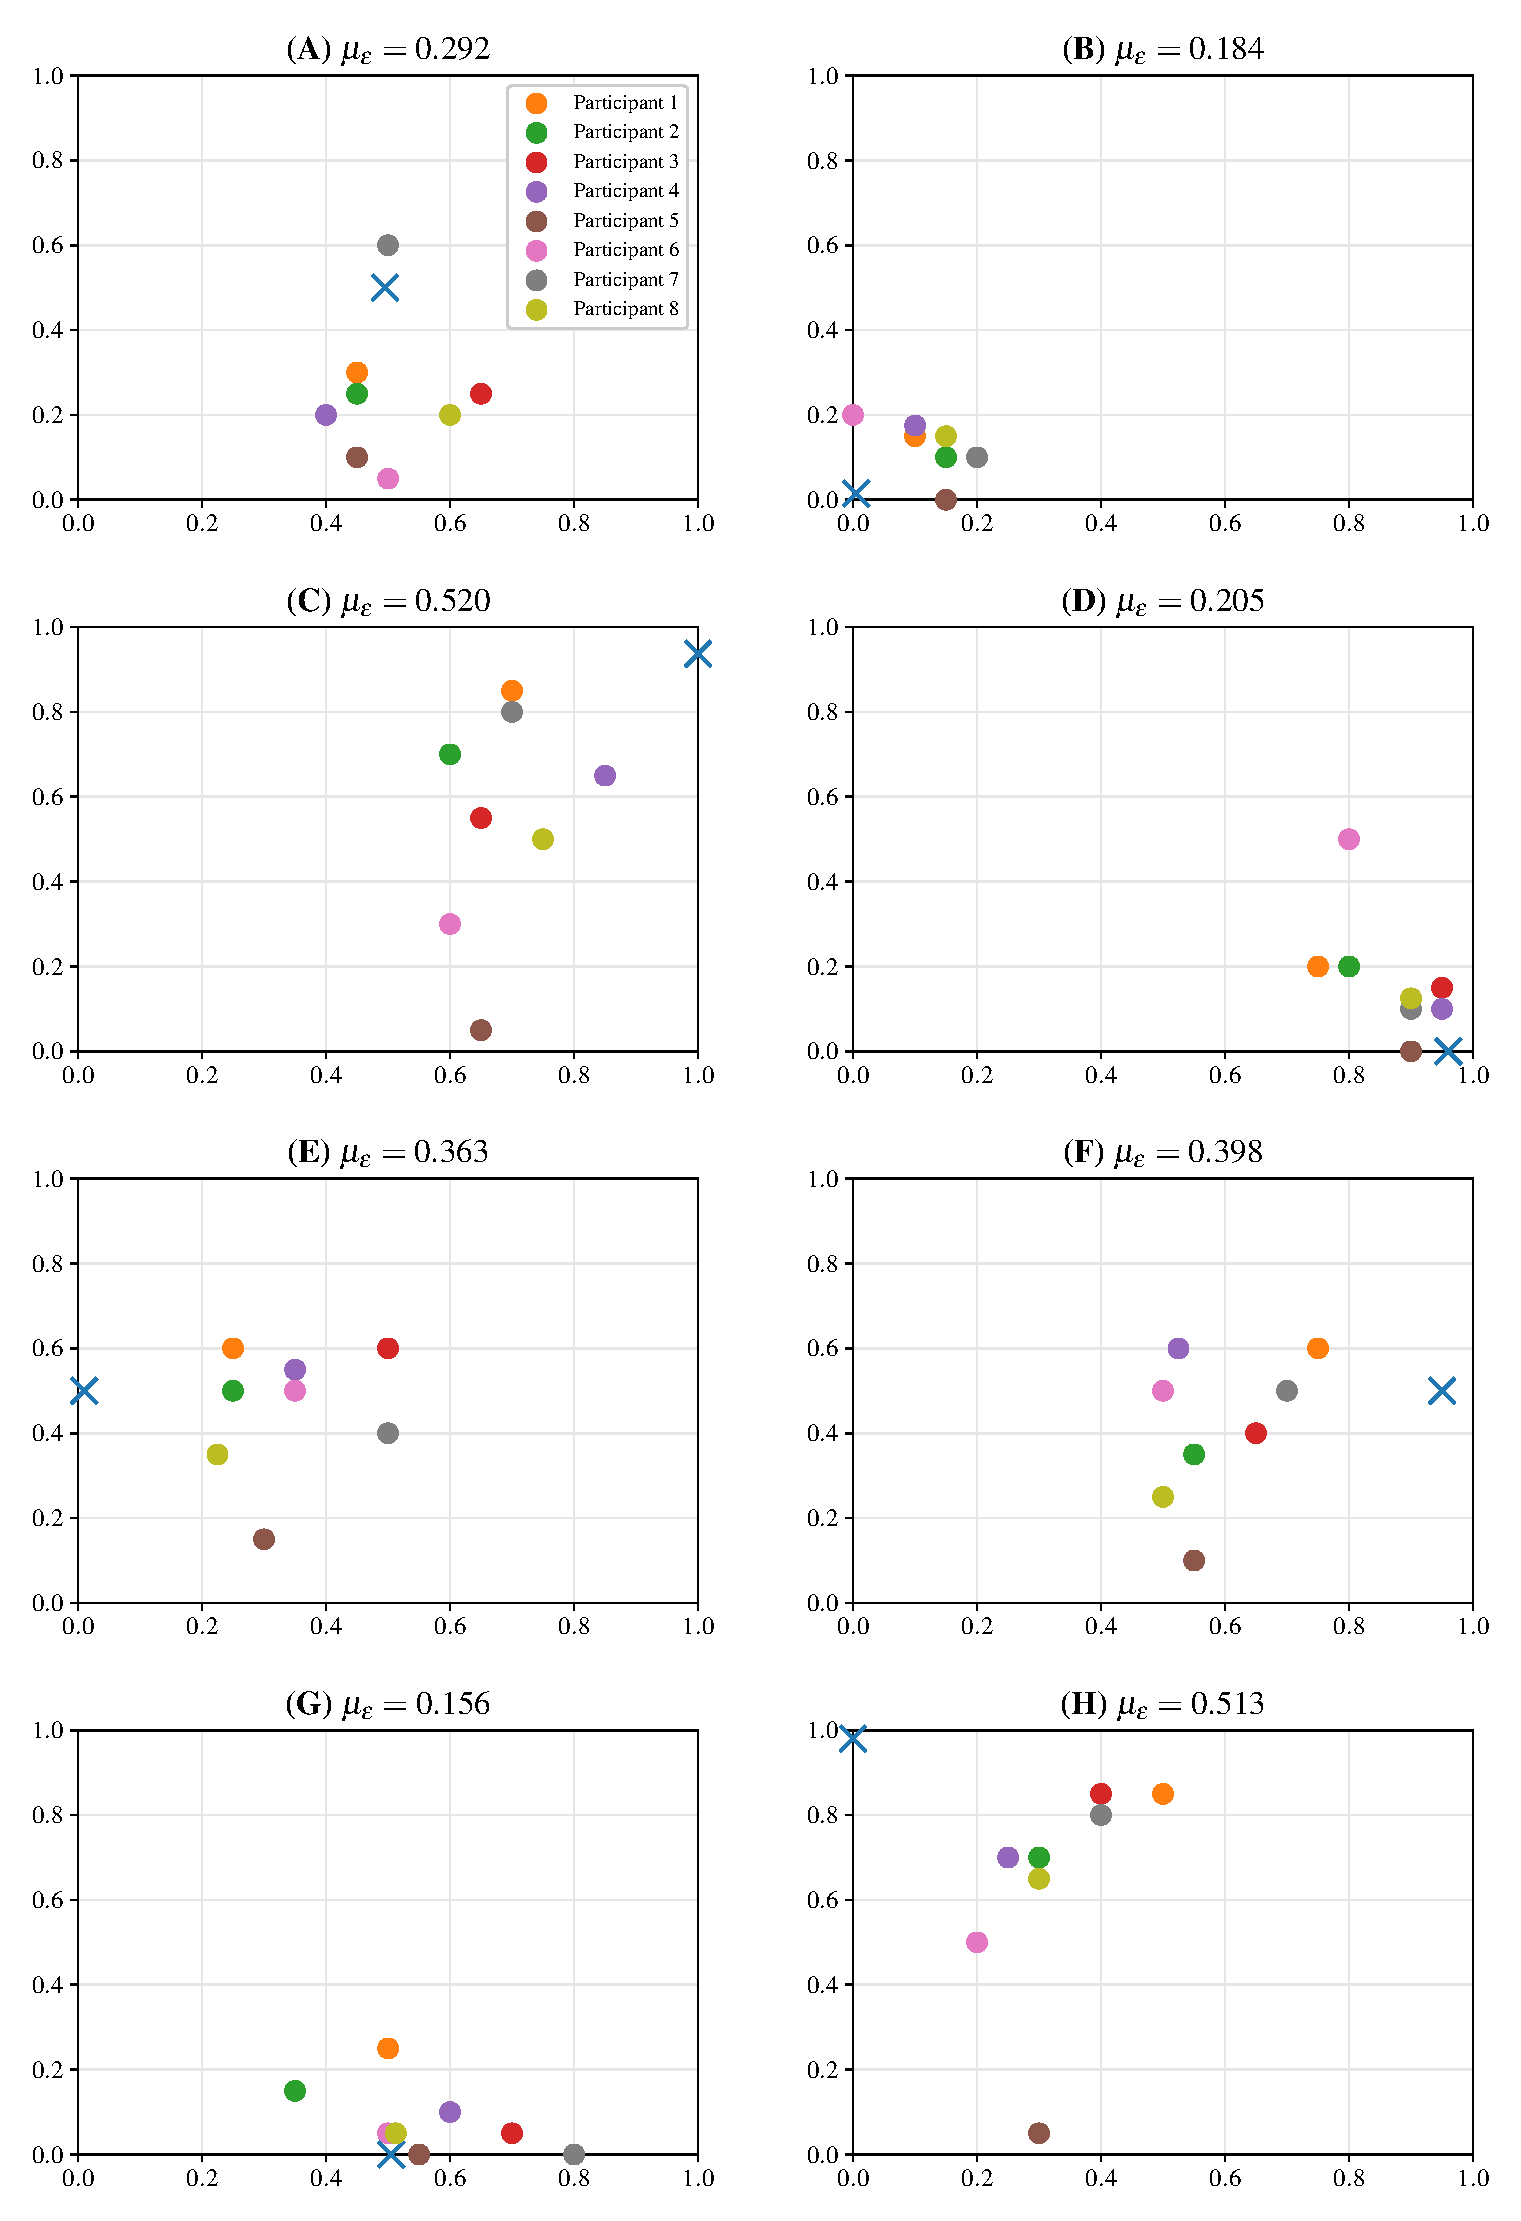
\includegraphics[width=.775\textwidth]{figures/subjective}
    \caption{
        Results of the perceptual evaluation.
        Lateral (horizontal axis) and longitudinal (vertical axis) components
        are normalised to $[0, 1]$.
        For each plot, the horizontal axis (i.e. longitudinal component
        equalling 0) corresponds with the location of the speaker array.
        Each plot shows the intended position of the virtual sound source as
        specified by parameters to the WFS plugin interface (cross) and
        estimated sound source positions as reported by participants (dots).
        Each plot is labelled with the mean Euclidean error $\mu_\epsilon$
        between intended position and reported positions.
        Legend in plot \textbf{(A)} applies to all plots.
    }
    \label{fig:perceptual}
\end{figure}

As can be seen, although far from perfect, and with some significant
outliers (e.g.\ the position reported by the fifth participant for test
\textbf{(D)}), certain trends do appear to emerge from the results.
Firstly, responses seem to loosely track the intended positions, with reported
positions most closely corresponding with intended ones for virtual source
locations lying close to the speaker array.
Indeed, tests \textbf{(B)}, \textbf{(D)}, and \textbf{(G)} exhibit the lowest
mean error values between the intended and reported positions.
The results for tests \textbf{(C)} and \textbf{(H)}, exhibit the greatest mean
error, and ambiguity regarding the lateral position of distant sound sources is
perhaps to be expected;
as the distance of a sound source from the listener increases, $r_k - y_k$
tends towards zero, and thus the ITD (and ILD) also approaches zero;
thus, with increased distance the wavefront produced by a sound source (be it a
real sound source or one synthesised under ideal conditions) approximates more
and more closely a plane wave.
In any case, despite this inherent, physical ambiguity, there is (visually
at least) a tendency amongst the results toward the lateral location of the
most longitudinally distant intended virtual source positions.
Particularly for test \textbf{(C)}, participants seem to have had greater
difficulty in estimating the depth of the virtual sound field; this may simply
be as a function of their developing a familiarity with that aspect of it over
the course of what was only a brief experiment.

Participants were asked for any anecdotal observations they had, based on their
experience of the experiment.
One participant noted, for the first position in particular, that the amplitude
variations between the snare drum strikes gave the impression of a sound source
that was advancing upon the listening position; for the lack of any visual cue
as to the position of the sound source, this is a reasonable conclusion to draw;
it did not, however, ultimately prevent them from reaching a decision with
regard to their estimate for the position of the sound source.
Another, likely hearing the time-varying comb-filter effect, asked whether the
``phasing'' they were hearing was intentional.
A third, also perceiving a similar phenomenon, suggested that they
felt that the sound sources were moving.
Finally, a participant with prior experience working with WFS systems, remarked
that the distance effect (i.e.\ the WFS prefilter) was perhaps a little extreme,
and not altogether realistic.

\subsection{Discussion}\label{subsec:discussion}

The temporal clustering and polarisation seen in
\figsref{fig:rtt-drift-16}{fig:rtt-drift-32} is indicative of two points for
concern with regard to technical implementation:
the read-write difference threshold strategy may be insufficiently forgiving,
forcing the read position into deleteriously fluctuating increment changes in
response to periods of jitter.
And without a master clock to indicate to each client the beginning of each
output audio block, even with clock rates perfectly aligned, there is nothing
to guarantee agreement of the timing of audio interrupts at the client side.

To avoid sudden, large or `unrealistic' clock adjustments, clients assess
the drift ratio as assessed via the ratio of network packet
transmission to reception and, if it lies beyond an arbitrary threshold,
simply resets the clock to the default \qty{44.1}{\kHz}.
Resets of this sort may account for the large steps seen in the drift plots
in \figsref{fig:rtt-drift-16}{fig:rtt-drift-32}.
It is clear that this strategy could be significantly improved upon.

The phasing effect noted by one participant is a  consequence of the approach
taken to combating jitter and keeping the clients close, temporally, together,
and as close to the server as possible.
It is clear that the current approach is, at best, too aggressive to be viable
for high-quality audio output.
Furthermore, an unpitched sound source like a snare drum, though audibly
susceptible to the time-varying comb-filter effect described, masks other
artefacts caused by phenomena such as rapid fluctuations in the clients' buffer
read position increment, and sudden, comparatively large audio clock
adjustments.

The above being said, the perceptual test shows that the system produces virtual
sound sources that listeners are, at least to some extent, able to localise.
Further, it achieves this at a significantly lower cost-per-channel than any of
the systems discussed in sections \secref{subsubsec:spatial-sota}, and, speakers
excepted, compares favourably with the OTTOSonics system referred to in
\secref{subsec:distributed-audio-systems}, particularly as channel-count
increases, i.e.\ in terms of cost, it has the potential to scale better.
The most costly component of the system is the computer, but this could be
exchanged for any interested user's personal machine, so long as it is able to
run a DAW and has an ethernet interface.
The Teensy modules, including audio shield, cost around \texteuro{45};
eight-port ethernet switches can be purchased for as little as \texteuro{20-30}
Assuming a computer costing \texteuro{1500}, at 16 channels we can estimate
around \texteuro{120}/channel, dropping to \texteuro{50} for 64 channels.


    \section{Discussion}\label{sec:discussion}


%    \section{Introduction}

For Original Research Articles \citep{conference}, Clinical Trial Articles \citep{article}, and Technology Reports \citep{patent}, the introduction should be succinct, with no subheadings \citep{book}. For Case Reports the Introduction should include symptoms at presentation \citep{chapter}, physical exams and lab results \citep{dataset}.


\section{Article types}

For requirements for a specific article type please refer to the Article Types on any Frontiers journal page. Please also refer to  \href{http://home.frontiersin.org/about/author-guidelines#Sections}{Author Guidelines} for further information on how to organize your manuscript in the required sections or their equivalents for your field

% For Original Research articles, please note that the Material and Methods section can be placed in any of the following ways: before Results, before Discussion or after Discussion.


\section{Manuscript Formatting}

\subsection{Heading Levels}

%There are 5 heading levels

\subsection{Level 2}

\subsubsection{Level 3}

\paragraph{Level 4}

\subparagraph{Level 5}

\subsection{Equations}
Equations should be inserted in editable format from the equation editor.

\begin{equation}
    \sum x+ y =Z\label{eq:01}
\end{equation}

\subsection{Figures}
Frontiers requires figures to be submitted individually, in the same order as they are referred to in the manuscript. Figures will then be automatically embedded at the bottom of the submitted manuscript. Kindly ensure that each table and figure is mentioned in the text and in numerical order. Figures must be of sufficient resolution for publication \href{https://www.frontiersin.org/about/author-guidelines#ImageSizeRequirements}{see here for examples and minimum requirements}. Figures which are not according to the guidelines will cause substantial delay during the production process. Please see \href{https://www.frontiersin.org/about/author-guidelines#FigureRequirementsStyleGuidelines}{here} for full figure guidelines. Cite figures with subfigures as figure \ref{fig:Subfigure 1} and \ref{fig:Subfigure 2}.

\subsubsection{Permission to Reuse and Copyright}
Figures, tables, and images will be published under a Creative Commons CC-BY licence and permission must be obtained for use of copyrighted material from other sources (including re-published/adapted/modified/partial figures and images from the internet). It is the responsibility of the authors to acquire the licenses, to follow any citation instructions requested by third-party rights holders, and cover any supplementary charges.
%%Figures, tables, and images will be published under a Creative Commons CC-BY licence and permission must be obtained for use of copyrighted material from other sources (including re-published/adapted/modified/partial figures and images from the internet). It is the responsibility of the authors to acquire the licenses, to follow any citation instructions requested by third-party rights holders, and cover any supplementary charges.

\subsection{Tables}
Tables should be inserted at the end of the manuscript. Please build your table directly in LaTeX.Tables provided as jpeg/tiff files will not be accepted. Please note that very large tables (covering several pages) cannot be included in the final PDF for reasons of space. These tables will be published as \href{http://home.frontiersin.org/about/author-guidelines#SupplementaryMaterial}{Supplementary Material} on the online article page at the time of acceptance. The author will be notified during the typesetting of the final article if this is the case.

\subsection{International Phonetic Alphabet}
To include international phonetic alphabet (IPA) symbols, please include the following functions:
Under useful packages, include:\begin{verbatim}\usepackage{tipa}
\end{verbatim}
In the main text, when inputting symbols, use the following format:\begin{verbatim}\text[symbolname]
\end{verbatim}e.g.\begin{verbatim}\textgamma
\end{verbatim}


\section{Nomenclature}

\subsection{Resource Identification Initiative}
To take part in the Resource Identification Initiative, please use the corresponding catalog number and RRID in your current manuscript. For more information about the project and for steps on how to search for an RRID, please click \href{http://www.frontiersin.org/files/pdf/letter_to_author.pdf}{here}.

\subsection{Life Science Identifiers}
Life Science Identifiers (LSIDs) for ZOOBANK registered names or nomenclatural acts should be listed in the manuscript before the keywords. For more information on LSIDs please see \href{https://www.frontiersin.org/about/author-guidelines#Nomenclature}{Inclusion of Zoological Nomenclature} section of the guidelines.


\section{Additional Requirements}

For additional requirements for specific article types and further information please refer to \href{http://www.frontiersin.org/about/AuthorGuidelines#AdditionalRequirements}{Author Guidelines}.

\section*{Conflict of Interest Statement}
%All financial, commercial or other relationships that might be perceived by the academic community as representing a potential conflict of interest must be disclosed. If no such relationship exists, authors will be asked to confirm the following statement:

The authors declare that the research was conducted in the absence of any commercial or financial relationships that could be construed as a potential conflict of interest.

\section*{Author Contributions}

The Author Contributions section is mandatory for all articles, including articles by sole authors. If an appropriate statement is not provided on submission, a standard one will be inserted during the production process. The Author Contributions statement must describe the contributions of individual authors referred to by their initials and, in doing so, all authors agree to be accountable for the content of the work. Please see  \href{https://www.frontiersin.org/about/policies-and-publication-ethics#AuthorshipAuthorResponsibilities}{here} for full authorship criteria.

\section*{Funding}
Details of all funding sources should be provided, including grant numbers if applicable. Please ensure to add all necessary funding information, as after publication this is no longer possible.

\section*{Acknowledgments}
This is a short text to acknowledge the contributions of specific colleagues, institutions, or agencies that aided the efforts of the authors.

\section*{Supplemental Data}
\href{http://home.frontiersin.org/about/author-guidelines#SupplementaryMaterial}{Supplementary Material} should be uploaded separately on submission, if there are Supplementary Figures, please include the caption in the same file as the figure. LaTeX Supplementary Material templates can be found in the Frontiers LaTeX folder.

\section*{Data Availability Statement}
The datasets [GENERATED/ANALYZED] for this study can be found in the [NAME OF REPOSITORY] [LINK].
% Please see the availability of data guidelines for more information, at https://www.frontiersin.org/about/author-guidelines#AvailabilityofData


    % As per https://www.frontiersin.org/Design/pdf/Frontiers_Journal_style_table.pdf
    \bibliographystyle{Frontiers-Harvard}
    \bibliography{NetworkedAudio}
    %%% Make sure to upload the bib file along with the tex file and PDF
    %%% Please see the test.bib file for some examples of references

%    \section*{Figure captions}

%%% Please be aware that for original research articles we only permit a
%%% combined number of 15 figures and tables, one figure with multiple
%%% subfigures will count as only one figure.
%%% Use this if adding the figures directly in the mansucript, if so, please
%%% remember to also upload the files when submitting your article
%%% There is no need for adding the file termination, as long as you indicate
%%% where the file is saved. In the examples below the files (logo1.eps and
%%% logos.eps) are in the Frontiers LaTeX folder
%%% If using *.tif files convert them to .jpg or .png
%%% NB logo1.eps is required in the path in order to correctly compile front
%%% page header

\begin{figure}[h!]
    \begin{center}
        
\includegraphics[width=10cm]{logo1}% This is a *.eps file
    \end{center}
    \caption{ Enter the caption for your figure here. Repeat as necessary for each of your figures}\label{fig:1}
\end{figure}

\setcounter{figure}{2}
\setcounter{subfigure}{0}
\begin{subfigure}
    \setcounter{figure}{2}
    \setcounter{subfigure}{0}
    \centering
    \begin{minipage}[b]{0.5\textwidth}
        
\includegraphics[width=\linewidth]{logo1.eps}
        \caption{This is Subfigure 1.}
        \label{fig:Subfigure 1}
    \end{minipage}

    \setcounter{figure}{2}
    \setcounter{subfigure}{1}
    \begin{minipage}[b]{0.5\textwidth}
        
\includegraphics[width=\linewidth]{logo2.eps}
        \caption{This is Subfigure 2.}
        \label{fig:Subfigure 2}
    \end{minipage}

    \setcounter{figure}{2}
    \setcounter{subfigure}{-1}
    \caption{Enter the caption for your subfigure here. \textbf{(A)} This is the caption for Subfigure 1. \textbf{(B)} This is the caption for Subfigure 2.}
    \label{fig: subfigures}
\end{subfigure}

%%% If you don't add the figures in the LaTeX files, please upload them when
%%% submitting the article.
%%% Frontiers will add the figures at the end of the provisional pdf
%%% automatically.
%%% The use of LaTeX coding to draw Diagrams/Figures/Structures should be
%%% avoided. They should be external callouts including graphics.


\end{document}
